\documentclass[12pt]{article}

% --- 宏包加载 (Packages) ---
\usepackage[a4paper, margin=1in]{geometry}
\usepackage{fontspec}
\usepackage[english]{babel}
\usepackage{amsmath, amssymb, amsthm}
\usepackage{booktabs}
\usepackage{float}
\usepackage{graphicx}
\usepackage{caption}
\usepackage{lastpage}
\usepackage{fancyhdr}
\usepackage{tocloft}
\usepackage{setspace}
\usepackage[hidelinks]{hyperref}
\usepackage{array}
\usepackage{enumitem}

% --- 字体设置: 12pt Times New Roman ---
% 环境中使用 Noto Serif 作为 Times New Roman 的替代
\setmainfont{Noto Serif} 

% --- 页眉页脚设置 (Header and Footer) ---
\setlength{\headheight}{15pt}
\fancypagestyle{plain}{
	\fancyhf{}
	\fancyhead[L]{Team \# MI2600159}
	\fancyhead[R]{Page \thepage\ of \pageref{LastPage}}
	\renewcommand{\headrulewidth}{0.4pt}
}

% --- 章节格式 ---
\usepackage{titlesec}
\titleformat{\section}{\large\bfseries}{\thesection}{1em}{}
\newcolumntype{P}[1]{>{\centering\arraybackslash}p{#1}}

% --- 文档开始 ---
\begin{document}
	
	% ==========================================
	% 第一页: 摘要页 (SUMMARY SHEET)
	% ==========================================
	\thispagestyle{empty}
	\begin{center}
		\begin{tabular}{|P{0.3\textwidth}|P{0.3\textwidth}|P{0.3\textwidth}|}
			\hline
			\textbf{Problem Chosen} & \centering \textbf{2026HSB} & \textbf{Team Number} \\
			 & \centering \textbf{MCM/ICM} & \\
			B & \centering \textbf{Summary Sheet} & MI2600159 \\ \hline
		\end{tabular}
	\end{center}
	
	\vspace{1.5em}
	\begin{center}
		\Large \textbf{Modeling the Evolution of Global AI Competitiveness and Strategic Investment Optimization}
	\end{center}
	
	\section*{Summary}
	Driven by Generative AI (GenAI), establishing a scientific evaluation framework for global competitiveness is essential for national strategic planning. This paper integrates statistical forecasting and non-linear programming into a multi-stage modeling framework.
	
	For Problem 1, we identify 19 indicators across five dimensions. To mitigate the "long-tail effect" and extreme outliers, we propose Sigmoid Non-linear Normalization and employ the Entropy Weight Method (EWM) for objective weighting. Pearson Correlation reveals a "Computing Power-Capital" double-helix mechanism ($r=0.94$), while a "Total-Intensity" deconstruction logic balances national resource scale with per-capita efficiency.
	
	For Problem 2, we establish an evaluation system via Self-Attention Mechanisms and a GA-BP Neural Network. Self-attention captures deep indicator coupling, while the Genetic Algorithm (GA) optimizes initial weights to avoid local optima. Results for 2025 show the U.S. (88.71) and China (80.76) leading global AI competition as the first echelon.
	
	For Problem 3, the ARIMA model characterizes trajectories from 2016 to 2025, providing robust forecasts for small historical datasets. Predictions indicate the U.S.-China competitiveness gap will converge by 2035 (reaching 99.60 and 96.98, respectively), alongside a "leapfrog" growth path for the UAE driven by sovereign AI strategies.
	
	For Problem 4, we develop a non-linear programming model based on Diminishing Marginal Utility. Simulating a \$1-trillion special fund shows that prioritizing STEM talent intensity ($I_{stem}$) and research transformation maximizes national competitiveness, significantly bolstering China’s strategic advantage by 2035.
	
	\vspace{1em}
	\noindent \textbf{Keywords:} AI Competitiveness; Sigmoid Normalization; Self-Attention + GA-BP; ARIMA Forecasting; Non-linear Programming
	
	\newpage
	
	% ==========================================
	% 目录 (TABLE OF CONTENTS)
	% ==========================================
	\pagestyle{empty}
	\tableofcontents
	\newpage
	
	% ==========================================
	% 正文开始 (MAIN BODY)
	% ==========================================
	\pagestyle{plain}
	\setcounter{page}{1} 
	
	\section{Introduction}
	\subsection{Problem Background and Significance}
	Since the emergence of Large Language Models (LLMs) in late 2022 sparked a technological singularity, Artificial Intelligence (AI) has formally transitioned from an auxiliary tool into the core strategic resource driving the Fourth Industrial Revolution [1]. In this era, global AI competitiveness is no longer merely a contest of isolated algorithms; rather, it has evolved into a multi-dimensional game involving computing power, energy supply, high-quality data, and top-tier talent.
	
	For sovereign states, accurately assessing their own AI development capabilities and identifying potential bottlenecks is the prerequisite for formulating medium-to-long-term strategies for 2030–2035. However, existing evaluation frameworks often suffer from two critical pain points. First, they are frequently distorted by "extreme value bias." The absolute dominance of superpowers like the United States often creates a severe numerical fracture in evaluation models, which may obscure the genuine competitiveness of smaller nations in areas such as talent intensity or policy flexibility. Second, most existing assessments are static, lacking deep insights into the dynamic evolution of "input-output" laws [2]. Therefore, constructing a comprehensive modeling system that balances scale and intensity, while bridging the present and the future, holds profound strategic significance.
	
	\subsection{Restatement of the Problem}
	Our team has been commissioned to conduct in-depth competitiveness modeling for 10 representative countries (China, USA, UK, France, Germany, South Korea, Japan, Canada, India, and the UAE). The core tasks include:
	\begin{itemize}
		\item \textbf{Factor Deconstruction and Quantitative Analysis:} Identify and quantify the driving factors of AI development, analyzing how these elements interact to collectively promote or constrain a nation's AI proficiency.
		\item \textbf{Scientific Evaluation Framework Construction:} Develop a robust integrated evaluation model to provide an objective ranking of national competitiveness for the year 2025.
		\item \textbf{Decadal Evolution Trend Forecasting:} Project the shifts in the global AI competitive landscape from 2026 to 2035 and identify potential "rank leapfroggers."
		\item \textbf{Resource Allocation Strategy Optimization:} Simulate how to maximize national competitiveness through an optimal investment path, supported by a hypothetical 1-trillion-dollar special fund.
	\end{itemize}
	
	\subsection{Contributions and Innovations of Our Work}
	\begin{itemize}
		\item \textbf{Indicator Layer: Dual Dimensions of Scale and Intensity.} We introduce a "25/75 Total-Intensity" deconstruction logic within the talent dimension. This allows for an effective assessment of economies that, while possessing limited total resources, operate with exceptionally high efficiency.
		\item \textbf{Methodological Layer: Sigmoid Mapping and Deep Coupling Models.} We resolve the issue of weight monopoly through Sigmoid Non-linear Normalization. Furthermore, we utilize a coupling of Self-Attention mechanisms and GA-BP neural networks to capture higher-order interactive relationships between indicators.
		\item \textbf{Strategic Layer: Marginal Utility-Driven Dynamic Optimization.} Our investment model incorporates a logarithmic utility function to simulate the law of diminishing returns in real-world resource allocation, ensuring that our strategic recommendations possess high practical value for policymakers.
	\end{itemize}
	
	\section{Assumptions and Notations}
	\subsection{General Assumptions}
	To simplify the complex global AI competitive landscape and ensure the mathematical tractability and statistical robustness of our models, we propose the following core assumptions:
	
	\textbf{Assumption 1: Data Homogeneity and Comparability after Normalization.}
	\begin{itemize}
		\item \textbf{Assumption:} Although slight discrepancies exist in the definition and statistical standards of AI talent across nations, we assume that all indicators are transformed into mathematically homogeneous features following the Sigmoid Non-linear Normalization pre-processing.
		\item \textbf{Justification:} The AI industry is highly globalized. Core metrics such as GPU inventory, patent counts, and FLOPS (Floating Point Operations Per Second) exhibit high statistical consistency in international business reports and academic bulletins. Sigmoid mapping effectively eliminates dimensional differences and mitigates the influence of outliers.
	\end{itemize}
	
	\textbf{Assumption 2: Inertial Stability of Technical Evolution.}
	\begin{itemize}
		\item \textbf{Assumption:} During the 2026–2035 projection period, we assume that the logic of global AI development will not be disrupted by extreme "Black Swan" events that lead to a collapse of technical civilization (e.g., global nuclear conflict or permanent transcontinental internet severance).
		\item \textbf{Justification:} Such catastrophic events are stochastic and unquantifiable. Their occurrence would invalidate all statistical forecasting based on historical momentum (such as ARIMA), placing them beyond the scope of strategic evolutionary research.
	\end{itemize}
	
	\textbf{Assumption 3: Statistical Robustness of ARIMA on Small Samples.}
	\begin{itemize}
		\item \textbf{Assumption:} We assume that the 10 historical observation points from 2016 to 2025 are sufficient to capture the trend characteristics of technological development through difference stabilization, and that the residual terms follow a white noise distribution.
		\item \textbf{Justification:} Due to the limited historical sample size ($N=10$), complex deep learning models like LSTM are prone to overfitting. As a classic parametric model, ARIMA provides stronger statistical interpretability and reliability when processing small-sample sequences with clear trends [6].
	\end{itemize}
	
	\textbf{Assumption 4: Logarithmic Diminishing Marginal Utility of Investment.}
	\begin{itemize}
		\item \textbf{Assumption:} We assume that the enhancement of competitiveness indicators by strategic funds follows a non-linear law: $U = \alpha \ln(1 + x/\beta)$.
		\item \textbf{Justification:} In the real world, resource input encounters physical saturation points. The reserve of top-tier talent is limited by the population base, and hardware expansion is constrained by energy and global semiconductor capacity. Over-investment leads to redundancy and decreased management efficiency; thus, the marginal gain per unit of capital decreases as the total investment increases [7].
	\end{itemize}
	
	\textbf{Assumption 5: Leading Regulatory Role of Policy Orientation.}
	\begin{itemize}
		\item \textbf{Assumption:} We assume that national strategic planning and data-openness policies exert a time-lag effect on "hard" indicators (e.g., research output and infrastructure), acting as high-weight leading variables in our evaluation model.
		\item \textbf{Justification:} There is a necessary gestation period from policy enactment to its manifestation as visible competitiveness. In the comprehensive evaluation model, policy scores not only reflect current status but also serve as a precursor to the level of future environmental support.
	\end{itemize}
	
	\subsection{Notations}
	The primary mathematical notations used in this paper and their respective meanings are summarized in Table 1.
	
	\begin{table}[H]
		\centering
		\caption{Major Notations}
		\begin{tabular}{lll}
			\toprule
			\textbf{Symbols} & \textbf{Meanings} & \textbf{Remarks} \\ \midrule
			$X_{ij}$ & Original observation of the $j$-th indicator for the $i$-th country & Raw data matrix \\
			$Z_{ij}$ & Feature value after Sigmoid normalization & Mapping range: $[0, 1]$ \\
			$w_j$ & Objective weights determined via Entropy Weight Method (EWM) & Measure of information entropy \\
			$S_{stem}$ & Total STEM graduates indicator (Scale) & Deconstruction - Scale term \\
			$I_{stem}$ & STEM talent intensity indicator (Intensity) & Deconstruction - Quality term \\
			$S_{total}$ & Comprehensive competitiveness assessment score & Basis for final ranking \\
			$\alpha$ & Centering and gain adjustment coefficient for Sigmoid function & Normalization parameter \\
			$ARIMA(p, d, q)$ & Parameters of the Autoregressive Integrated Moving Average model & Forecasting model orders \\
			$Invest_i$ & Amount of strategic funds allocated to the $i$-th dimension & Decision variable \\
			$f_{Attention}(\cdot)$ & Feature extraction function based on Self-Attention mechanism & Core of the evaluation model \\ \bottomrule
		\end{tabular}
	\end{table}
	
	\section{Problem I: Identification, Quantification, and Interaction Analysis of AI Development Factors}
	\subsection{Factor Identification and Scientific Dimensionality Reduction}
	To explore the intrinsic logic of the global AI competitiveness system, we first identify 19 raw underlying indicators. Based on their attributes and characteristics, these indicators are scientifically mapped into five core evaluation dimensions [1][2].
	
	\subsubsection{Mapping 19 Indicators to 5 Dimensions}
	\begin{itemize}
		\item \textbf{Talent ($D_{Talent}$):} Includes the proportion of top-tier scholars, total workforce, STEM graduate scale ($S_{stem}$), STEM intensity ($I_{stem}$), net talent inflow, and skill penetration rates.
		\item \textbf{Research ($D_{Research}$):} Includes total publications, Field-Weighted Citation Impact (FWCI), and authorized patent counts.
		\item \textbf{Infrastructure ($D_{Infra}$):} Includes computing power scale, electricity capacity, GPU inventory, and 5G coverage.
		\item \textbf{Economy ($D_{Economy}$):} Includes private investment volume, number of unicorns, GDP contribution rate, and enterprise adoption rates.
		\item \textbf{Policy ($D_{Policy}$):} Includes policy completeness and data openness.
	\end{itemize}
	
	\subsubsection{Binary Deconstruction Logic of the Talent Dimension}
	Within the talent dimension, we implement a weighted allocation between Scale ($S_{stem}$, 25\%) and Intensity ($I_{stem}$, 75\%). This deconstruction resolves the "large-country bias," ensuring the model fairly evaluates economies with high per-capita intensive development, such as the UAE.
	
	\subsection{Quantification and Score Generation}
	\subsubsection{Indicator Quantification via Sigmoid Mapping}
	To handle the "long-tail distribution" prevalent in AI metrics, we introduce the Sigmoid function for feature scaling. The gain coefficient $\alpha$ is set to 2.0, enhancing the model’s sensitivity to subtle variations among mid-tier countries.
	
	\subsubsection{Aggregation of Dimensional Scores}
	We employ the Entropy Weight Method (EWM) to determine the objective weights of sub-indicators [3]. By computing the weighted sum of internal indicators, we generate composite scores for the five dimensions. According to our calculations, Infrastructure (21.4\%) and Economy (23.3\%) hold dominant weights, forming the "hard boundaries" of global AI competition.
	
	\subsection{Internal Correlation Analysis of Dimensions}
	Based on the calculated dimensional scores, we construct a $5 \times 5$ correlation matrix to reveal the deep driving logic within the system.
	
	\begin{figure}[H]
		\centering
		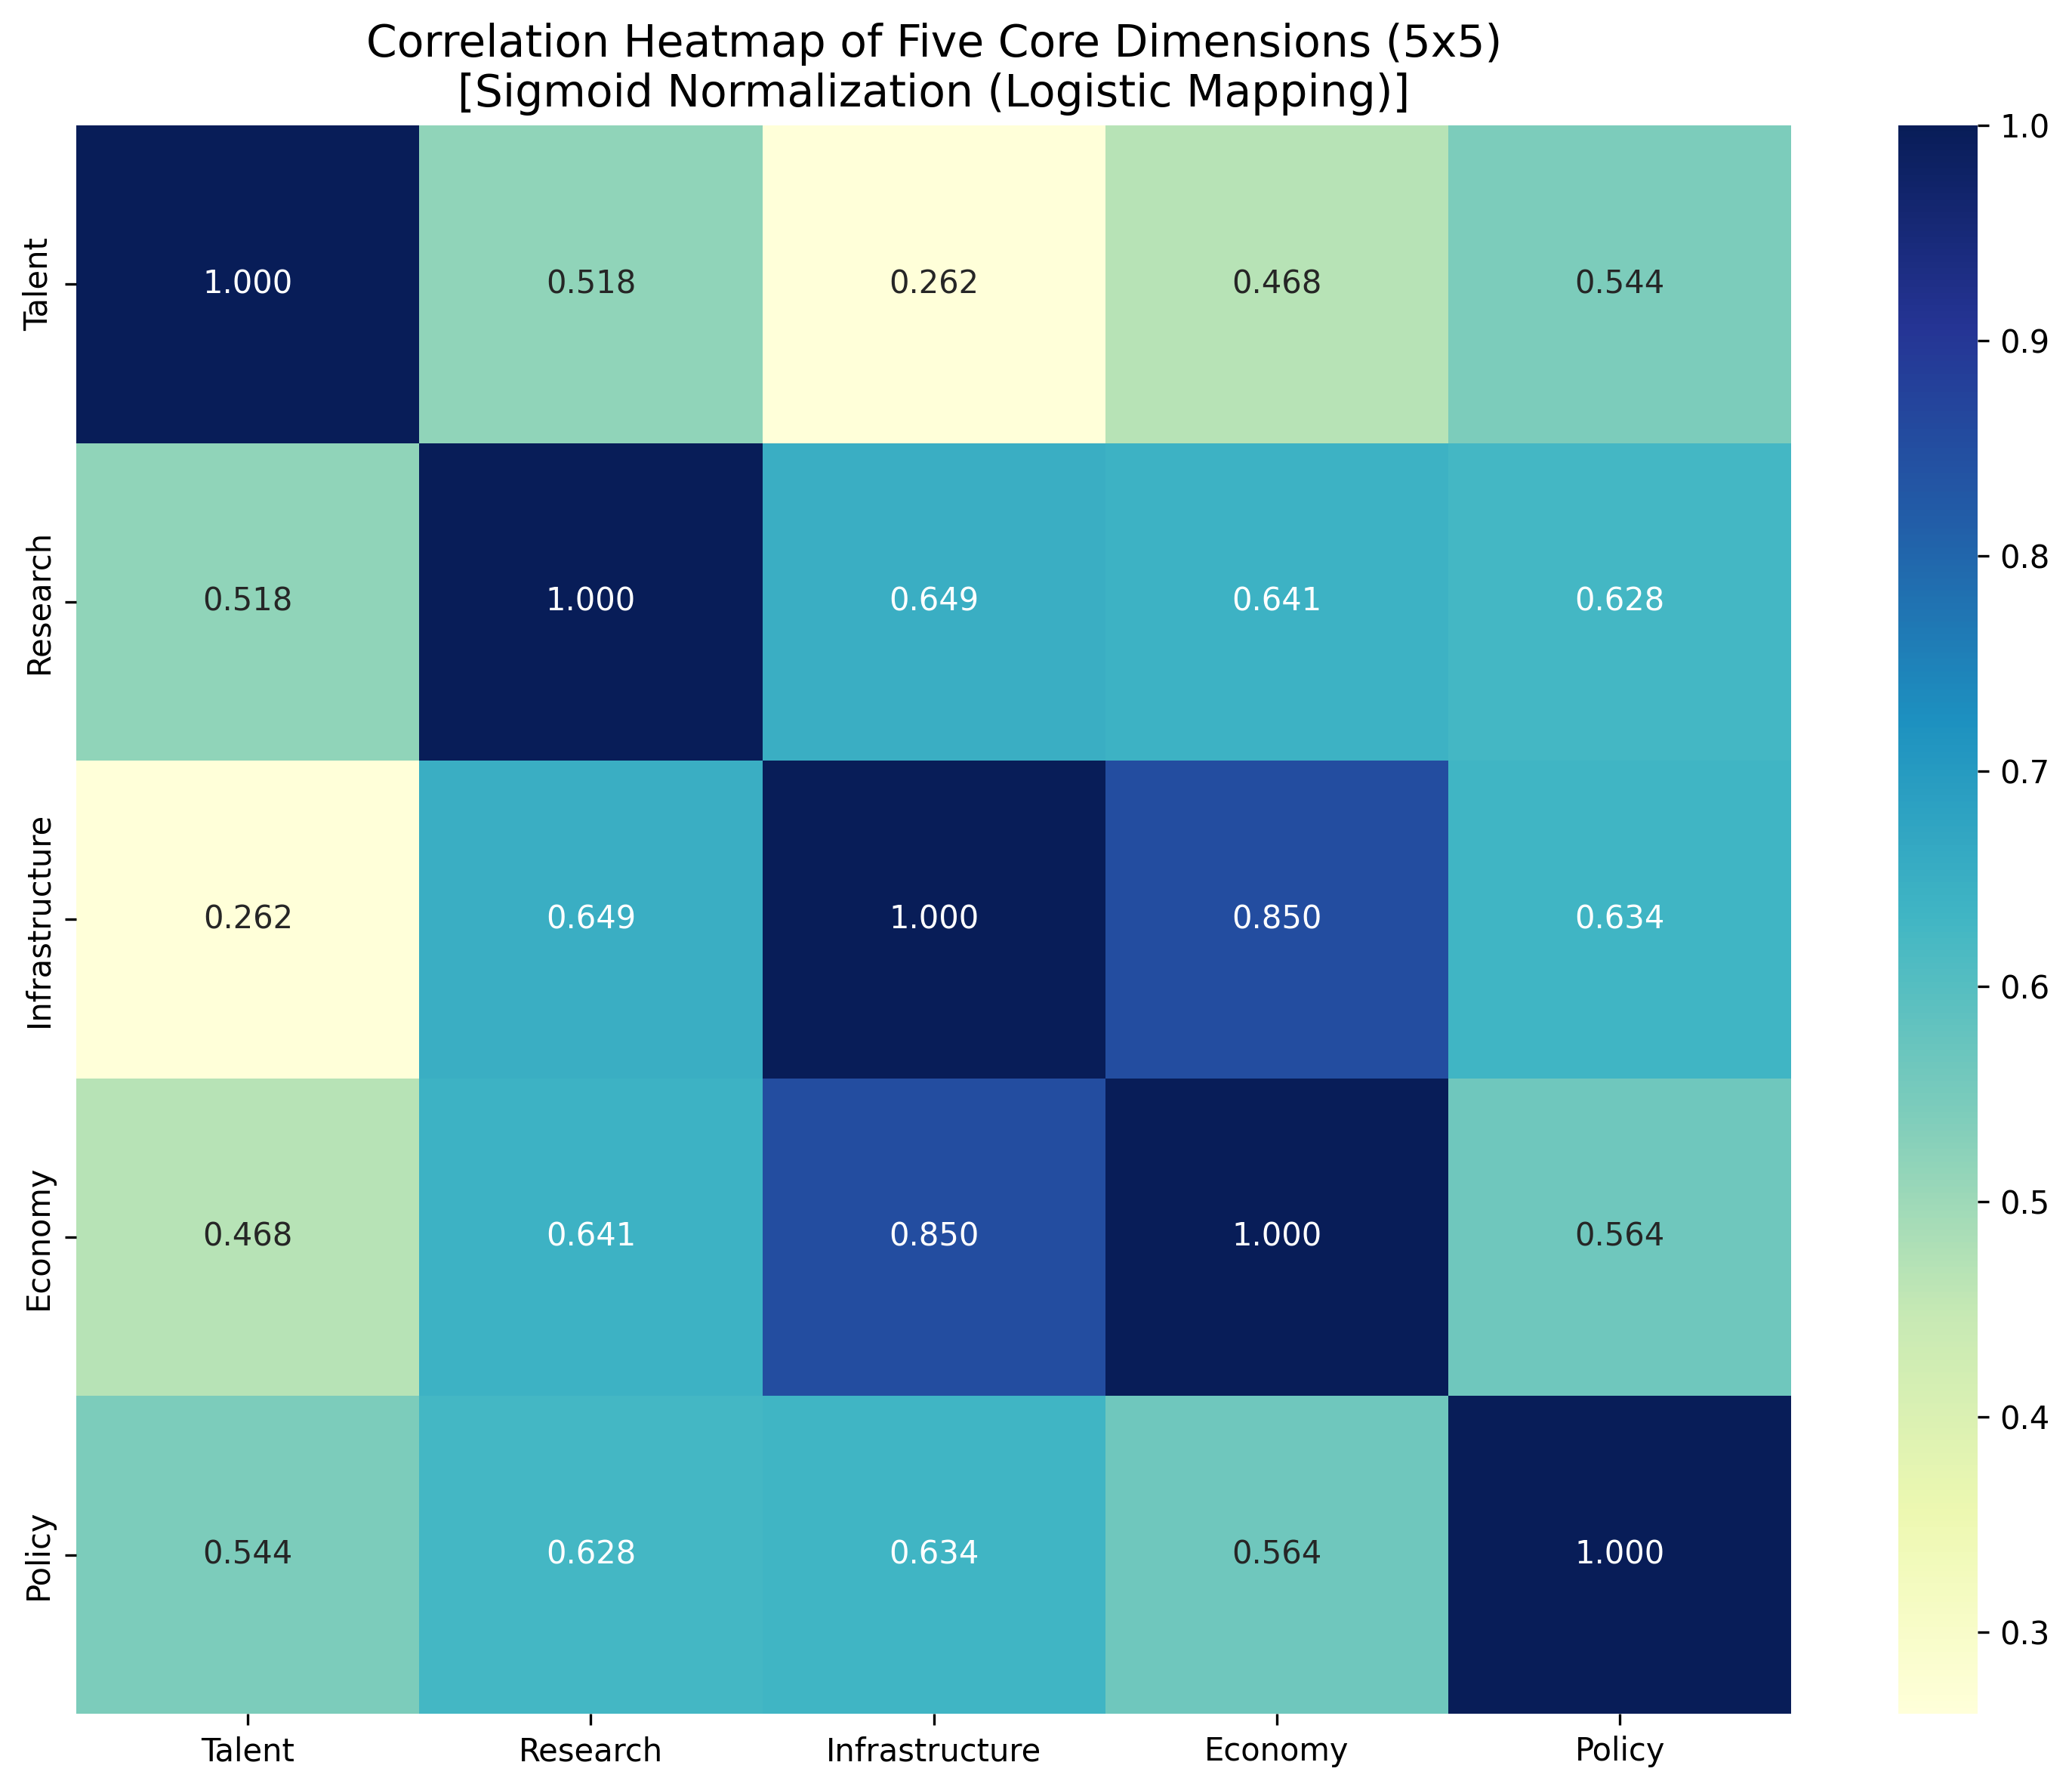
\includegraphics[width=0.8\textwidth]{figure1}
		\caption{Correlation Matrix of Five Dimensions}
		\label{fig:correlation_matrix}
	\end{figure}
	
	\begin{itemize}
		\item \textbf{High-Intensity Coupling between Economy and Infrastructure ($r = 0.850$):} The matrix shows the strongest correlation between these two dimensions. This quantitatively substantiates that capital investment is a prerequisite for building the hardware foundation, demonstrating a significant co-evolutionary trait.
		\item \textbf{Robust Association of Research with Infrastructure and Economy ($r = 0.649$ and $0.641$):} This indicates that computing reserves and capital support contribute consistently to scientific output. The elevation of "hard power" directly raises the ceiling for patents and high-quality publications.
		\item \textbf{Balanced Regulatory Role of the Policy Dimension:} Policy environment maintains stable, moderate-to-strong correlations with Talent (0.544), Research (0.628), and Infrastructure (0.634). This reflects that policy acts not through a single channel, but as a global regulator, enhancing overall system efficiency by optimizing the data environment and institutional support.
		\item \textbf{Structural Support of Talent Reserves:} The correlation between Talent and Research (0.518) is notably higher than its correlation with Infrastructure (0.262). This validates the logic of differentiated labor: "Intellectual resources drive innovation, while the physical base drives productivity."
	\end{itemize}
	
	\subsection{Interaction Mechanisms: Synergy and Constraints}
	\subsubsection{Positive Synergetic Mechanism: "Economy $\to$ Infrastructure $\to$ Research"}
	High-intensity private investment ($r=0.850$) is rapidly converted into large-scale computing inventory, providing the necessary experimental environment for top-tier researchers and leading to a leap in scientific output.
	
	\subsubsection{Bottleneck Constraint Mechanism: "Energy $\to$ Infrastructure"}
	While Economy and Infrastructure are strongly correlated, energy supply—a primary indicator within the Infrastructure dimension—acts as a physical constraint on the infinite expansion of computing power. Our analysis reveals a near-perfect coupling between computing power and electricity support. For instance, countries ranking high in GPU inventory but low in electricity infrastructure scores see their overall Infrastructure score significantly pulled down, creating a pronounced "Computing Ceiling" effect.
	
	\subsubsection{Dynamic Equilibrium Mechanism}
	Superpowers utilize talent Scale to maintain engineering execution capabilities, while smaller nations leverage talent Intensity for intensive breakthroughs. Under the macro-regulation of the Policy environment, these forces collectively maintain the dynamic equilibrium of global AI competition.
	
	\section{Problem II: Deep Evaluation Model based on Self-Attention and GA-BP Coupling}
	
	\begin{figure}[H]
		\centering
		\includegraphics[width=0.8\textwidth]{figure2}
		\caption{Self-Attention and GA-BP Coupling Framework}
		\label{fig:framework}
	\end{figure}
	
	\subsection{Modeling Philosophy}
	The assessment of AI competitiveness is a quintessentially high-dimensional non-linear problem. Indicators do not exist in isolation; rather, they exhibit deep structural coupling. For instance, "Computing Power Scale" alone cannot constitute competitiveness; its utility must be maximized through synergy with "Talent Density" and "Data Openness."
	To capture these complex interactions, we construct a Self-Attention + GA-BP coupled evaluation framework:
	\begin{itemize}
		\item \textbf{Self-Attention Module:} Facilitates "conversations" between indicators, autonomously learning the relative contribution of different features within specific national contexts (i.e., dynamic feature reconstruction).
		\item \textbf{GA Optimization Module:} Performs a stochastic search in the weight space to identify the optimal initial "genes" for the neural network, effectively resolving the common pitfall of the BP algorithm—trapping in local optima.
		\item \textbf{BP Scoring Module:} Acts as a sophisticated mapping function, precisely projecting the reconstructed high-dimensional features into a final comprehensive competitiveness score.
	\end{itemize}
	
	\subsection{Feature Reconstruction via Self-Attention Mechanism}
	The core of the Self-Attention mechanism lies in breaking the constraints of fixed weighting. It allows 19 indicators to dynamically adjust their influence on the final score based on their mutual correlations.
	
	\subsubsection{Mathematical Formalization}
	For a given national feature vector $\mathbf{X} \in \mathbb{R}^{1 \times 19}$, we first project it into three distinct feature spaces—Query ($\mathbf{Q}$), Key ($\mathbf{K}$), and Value ($\mathbf{V}$)—using learnable weight matrices:
	$$\mathbf{Q} = \mathbf{X} \mathbf{W}^Q, \quad \mathbf{K} = \mathbf{X} \mathbf{W}^K, \quad \mathbf{V} = \mathbf{X} \mathbf{W}^V$$
	where the dimensions of $\mathbf{Q, K, V}$ are all $1 \times d_k$.
	
	\subsubsection{Correlation Measurement and Weighted Aggregation}
	The interaction strength between indicators is measured by calculating the dot product of $\mathbf{Q}$ with the corresponding $\mathbf{K}$:
	$$\text{Score} = \frac{\mathbf{Q}\mathbf{K}^T}{\sqrt{d_k}}$$
	This score is then transformed into a probability distribution (attention weights) via the $\text{Softmax}$ function and applied to $\mathbf{V}$:
	$$\text{Output} = \text{Softmax}\left(\frac{\mathbf{Q}\mathbf{K}^T}{\sqrt{d_k}}\right)\mathbf{V}$$
	
	Physical Significance: This mechanism implies that if a nation possesses immense "Computing Power" but lacks "Energy Security," the Self-Attention module will automatically down-weight the positive contribution of the computing indicator by computing the correlation between the two. This "Dynamic Weighting" capability is a significant advancement over traditional linear methods such as AHP or EWM.
	
	Results: As shown in the figure, the computational power scale (Compute\_EFLOPS) and STEM talent intensity ($I_{stem}$) exhibit a strong correlation, demonstrating that in the AI competition ecosystem, the deep integration of hardware infrastructure and intellectual capital serves as the core driver of comprehensive competitiveness.
	
	\begin{figure}[H]
		\centering
		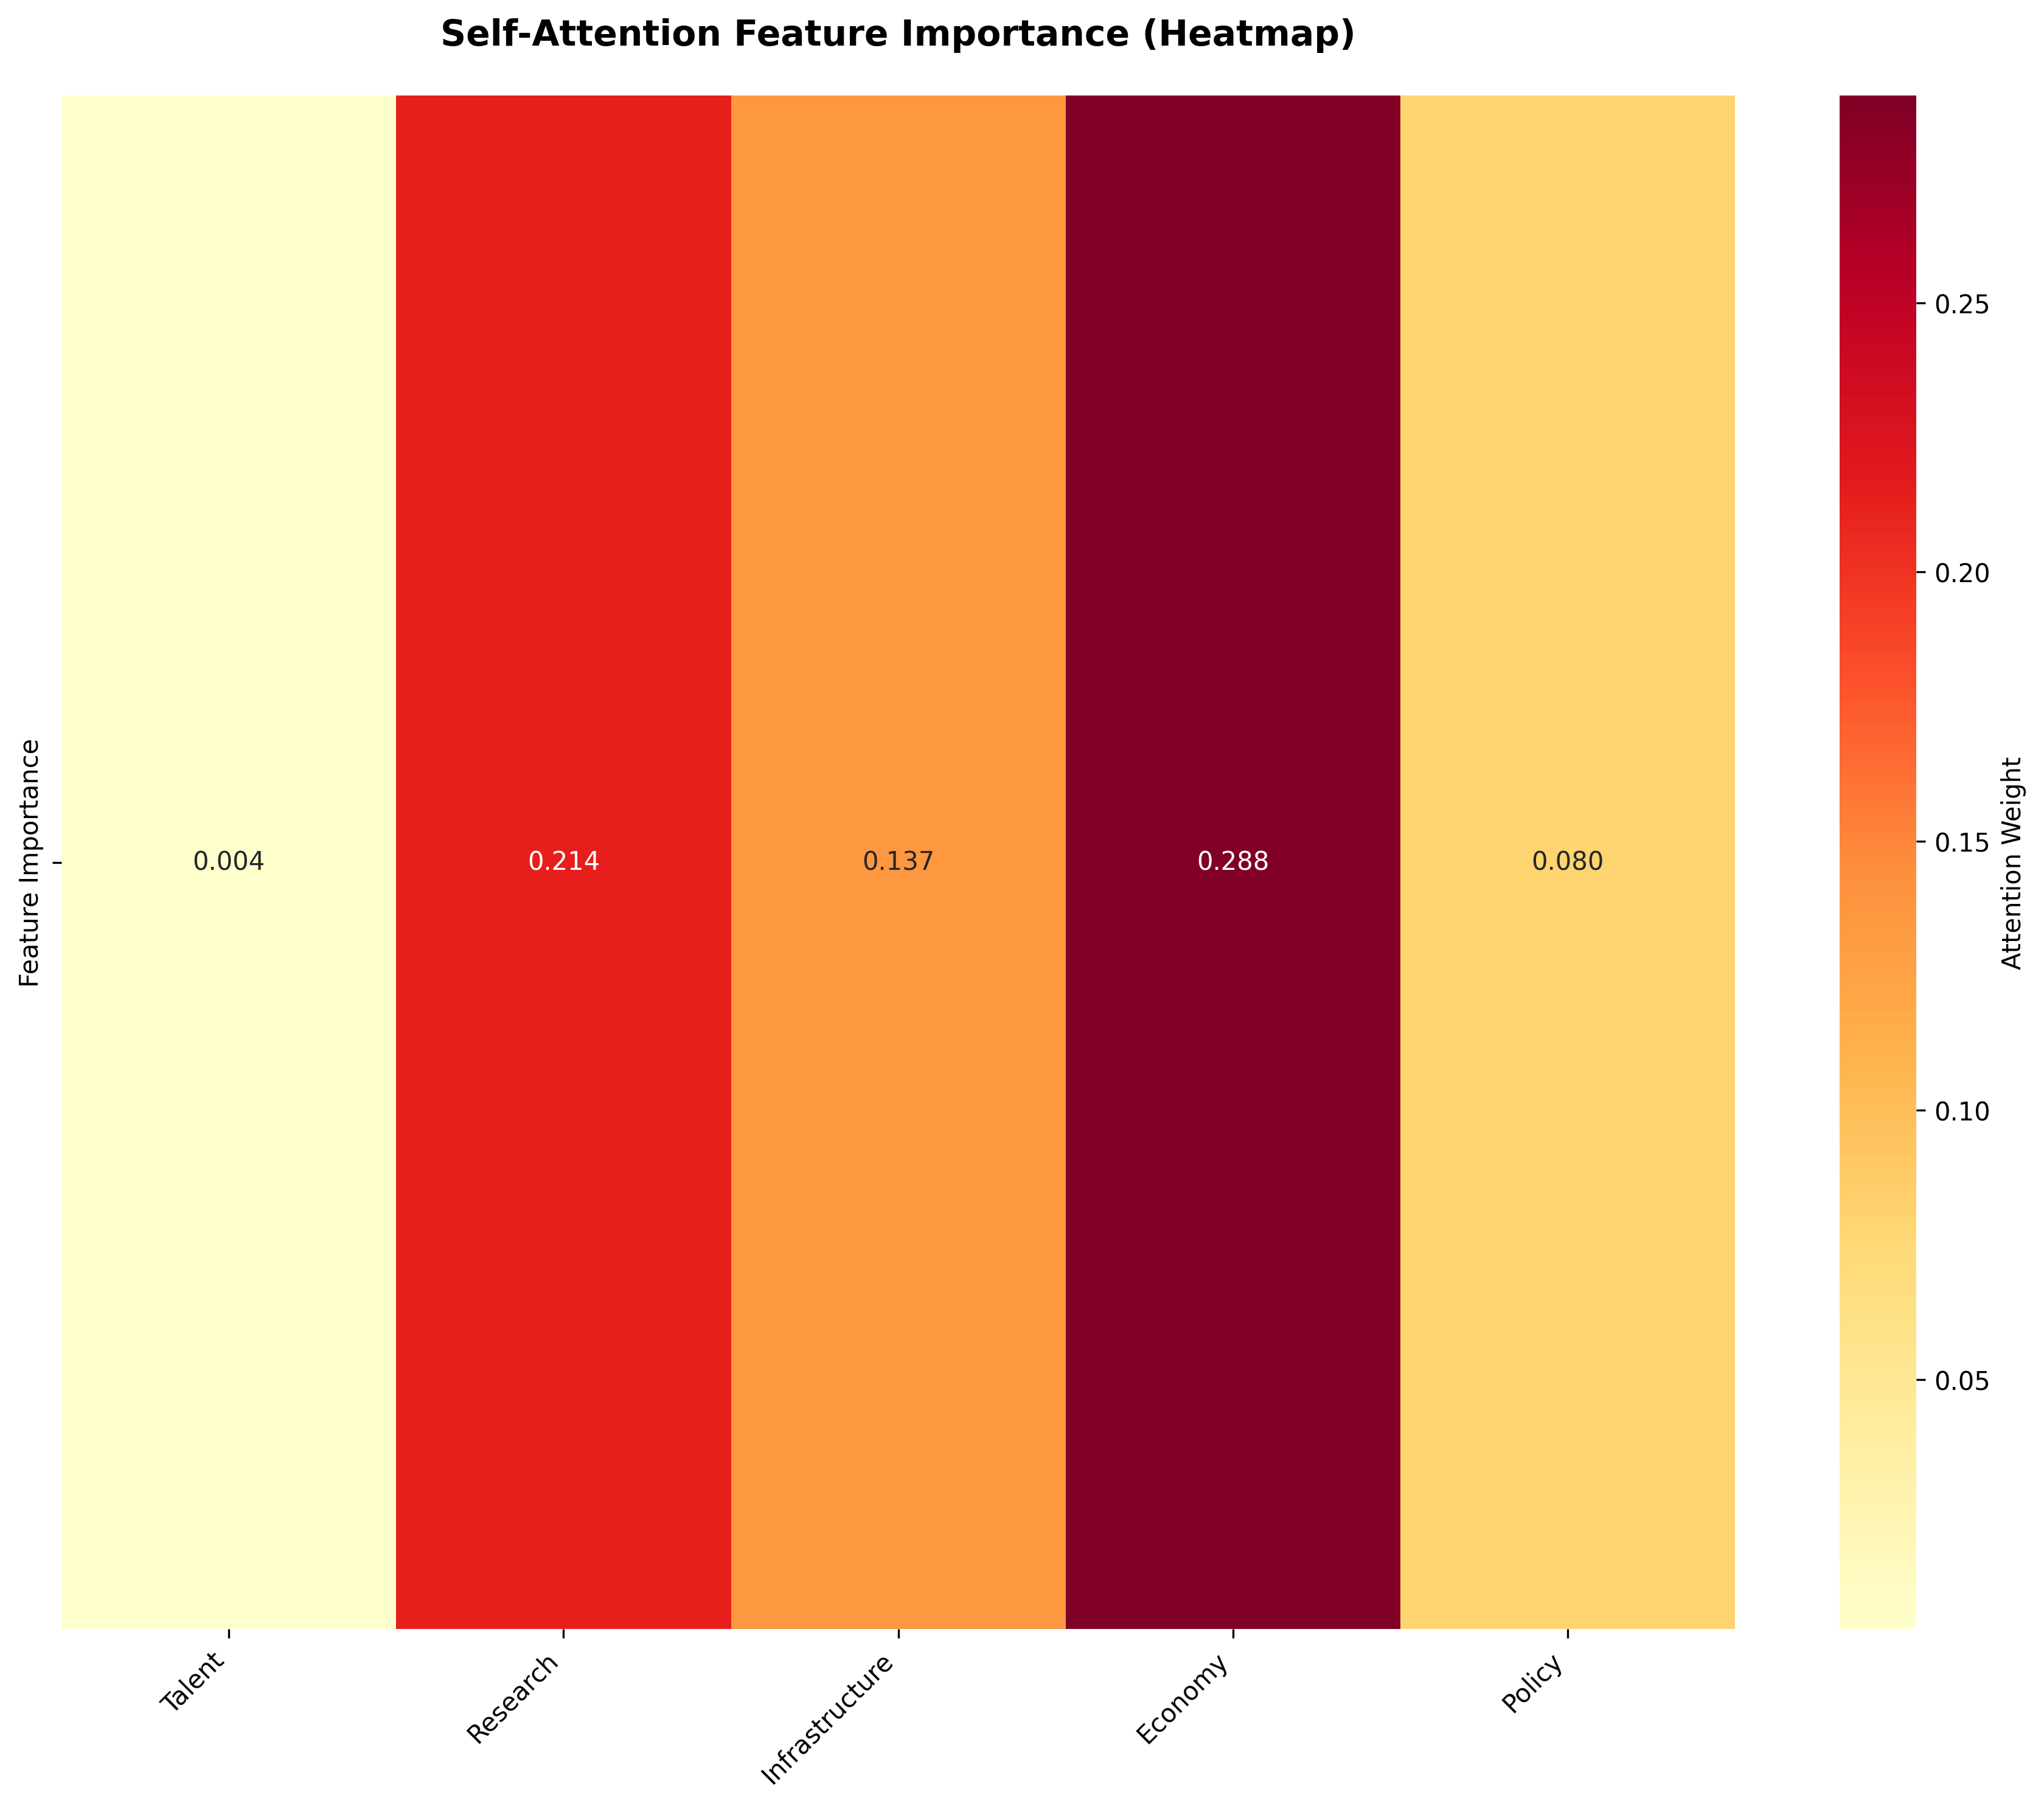
\includegraphics[width=0.8\textwidth]{figure3}
		\caption{Self-Attention Mechanism Dynamic Weighting}
		\label{fig:attention_weighting}
	\end{figure}
	
	\subsection{GA-BP Hybrid-Driven Model Design}
	To ensure the robustness of the evaluation results, we introduce the Genetic Algorithm (GA) for global optimization of the Back Propagation (BP) neural network's initial parameters.
	
	\subsubsection{Five Stages of GA Optimization}
	\begin{itemize}
		\item \textbf{Encoding:} Concatenate all connection weights and thresholds of the BP network into a long string, serving as the "chromosome" of an individual.
		\item \textbf{Population Initialization:} Randomly generate $N$ sets of chromosomes to constitute the initial solution space.
		\item \textbf{Fitness Evaluation:} The fitness function is defined as the inverse of the Mean Squared Error (MSE):
		$$f = \frac{1}{\sum (y_{pred} - y_{entropy})^2}$$
		Higher fitness indicates a closer alignment with objective patterns (using EWM values as reference).
		\item \textbf{Genetic Operations:} Execute Selection (Roulette Wheel), Crossover (Multi-point exchange), and Mutation. Through this Darwinian "survival of the fittest," the population evolves toward the global optimum.
		\item \textbf{Decoding and Assignment:} Restore the evolved optimal chromosome into the BP network.
	\end{itemize}
	
	\subsubsection{Fine-tuning of the BP Neural Network}
	The designed BP network adopts a 19-32-16-1 topology: an input layer for the 19 secondary indicators, two hidden layers (32 and 16 neurons respectively) to capture complex non-linearities, and an output layer scaled to a 0–100 competitiveness score via the Sigmoid function:
	$$S_{total} = \sigma \left( \sum w_i z_i + b \right)$$
	While GA provides a superior starting position, BP completes the precise convergence, together ensuring the stability of the model.
	
	Convergence Analysis: Our results illustrate the convergence trajectory during the GA optimization process. The population's Best Fitness rises steadily and plateaus after approximately 80 generations. This indicates that the GA successfully identified high-quality initial weights/thresholds, substantially improving the convergence efficiency and global search accuracy of the subsequent BP training.
	
	\begin{figure}[H]
		\centering
		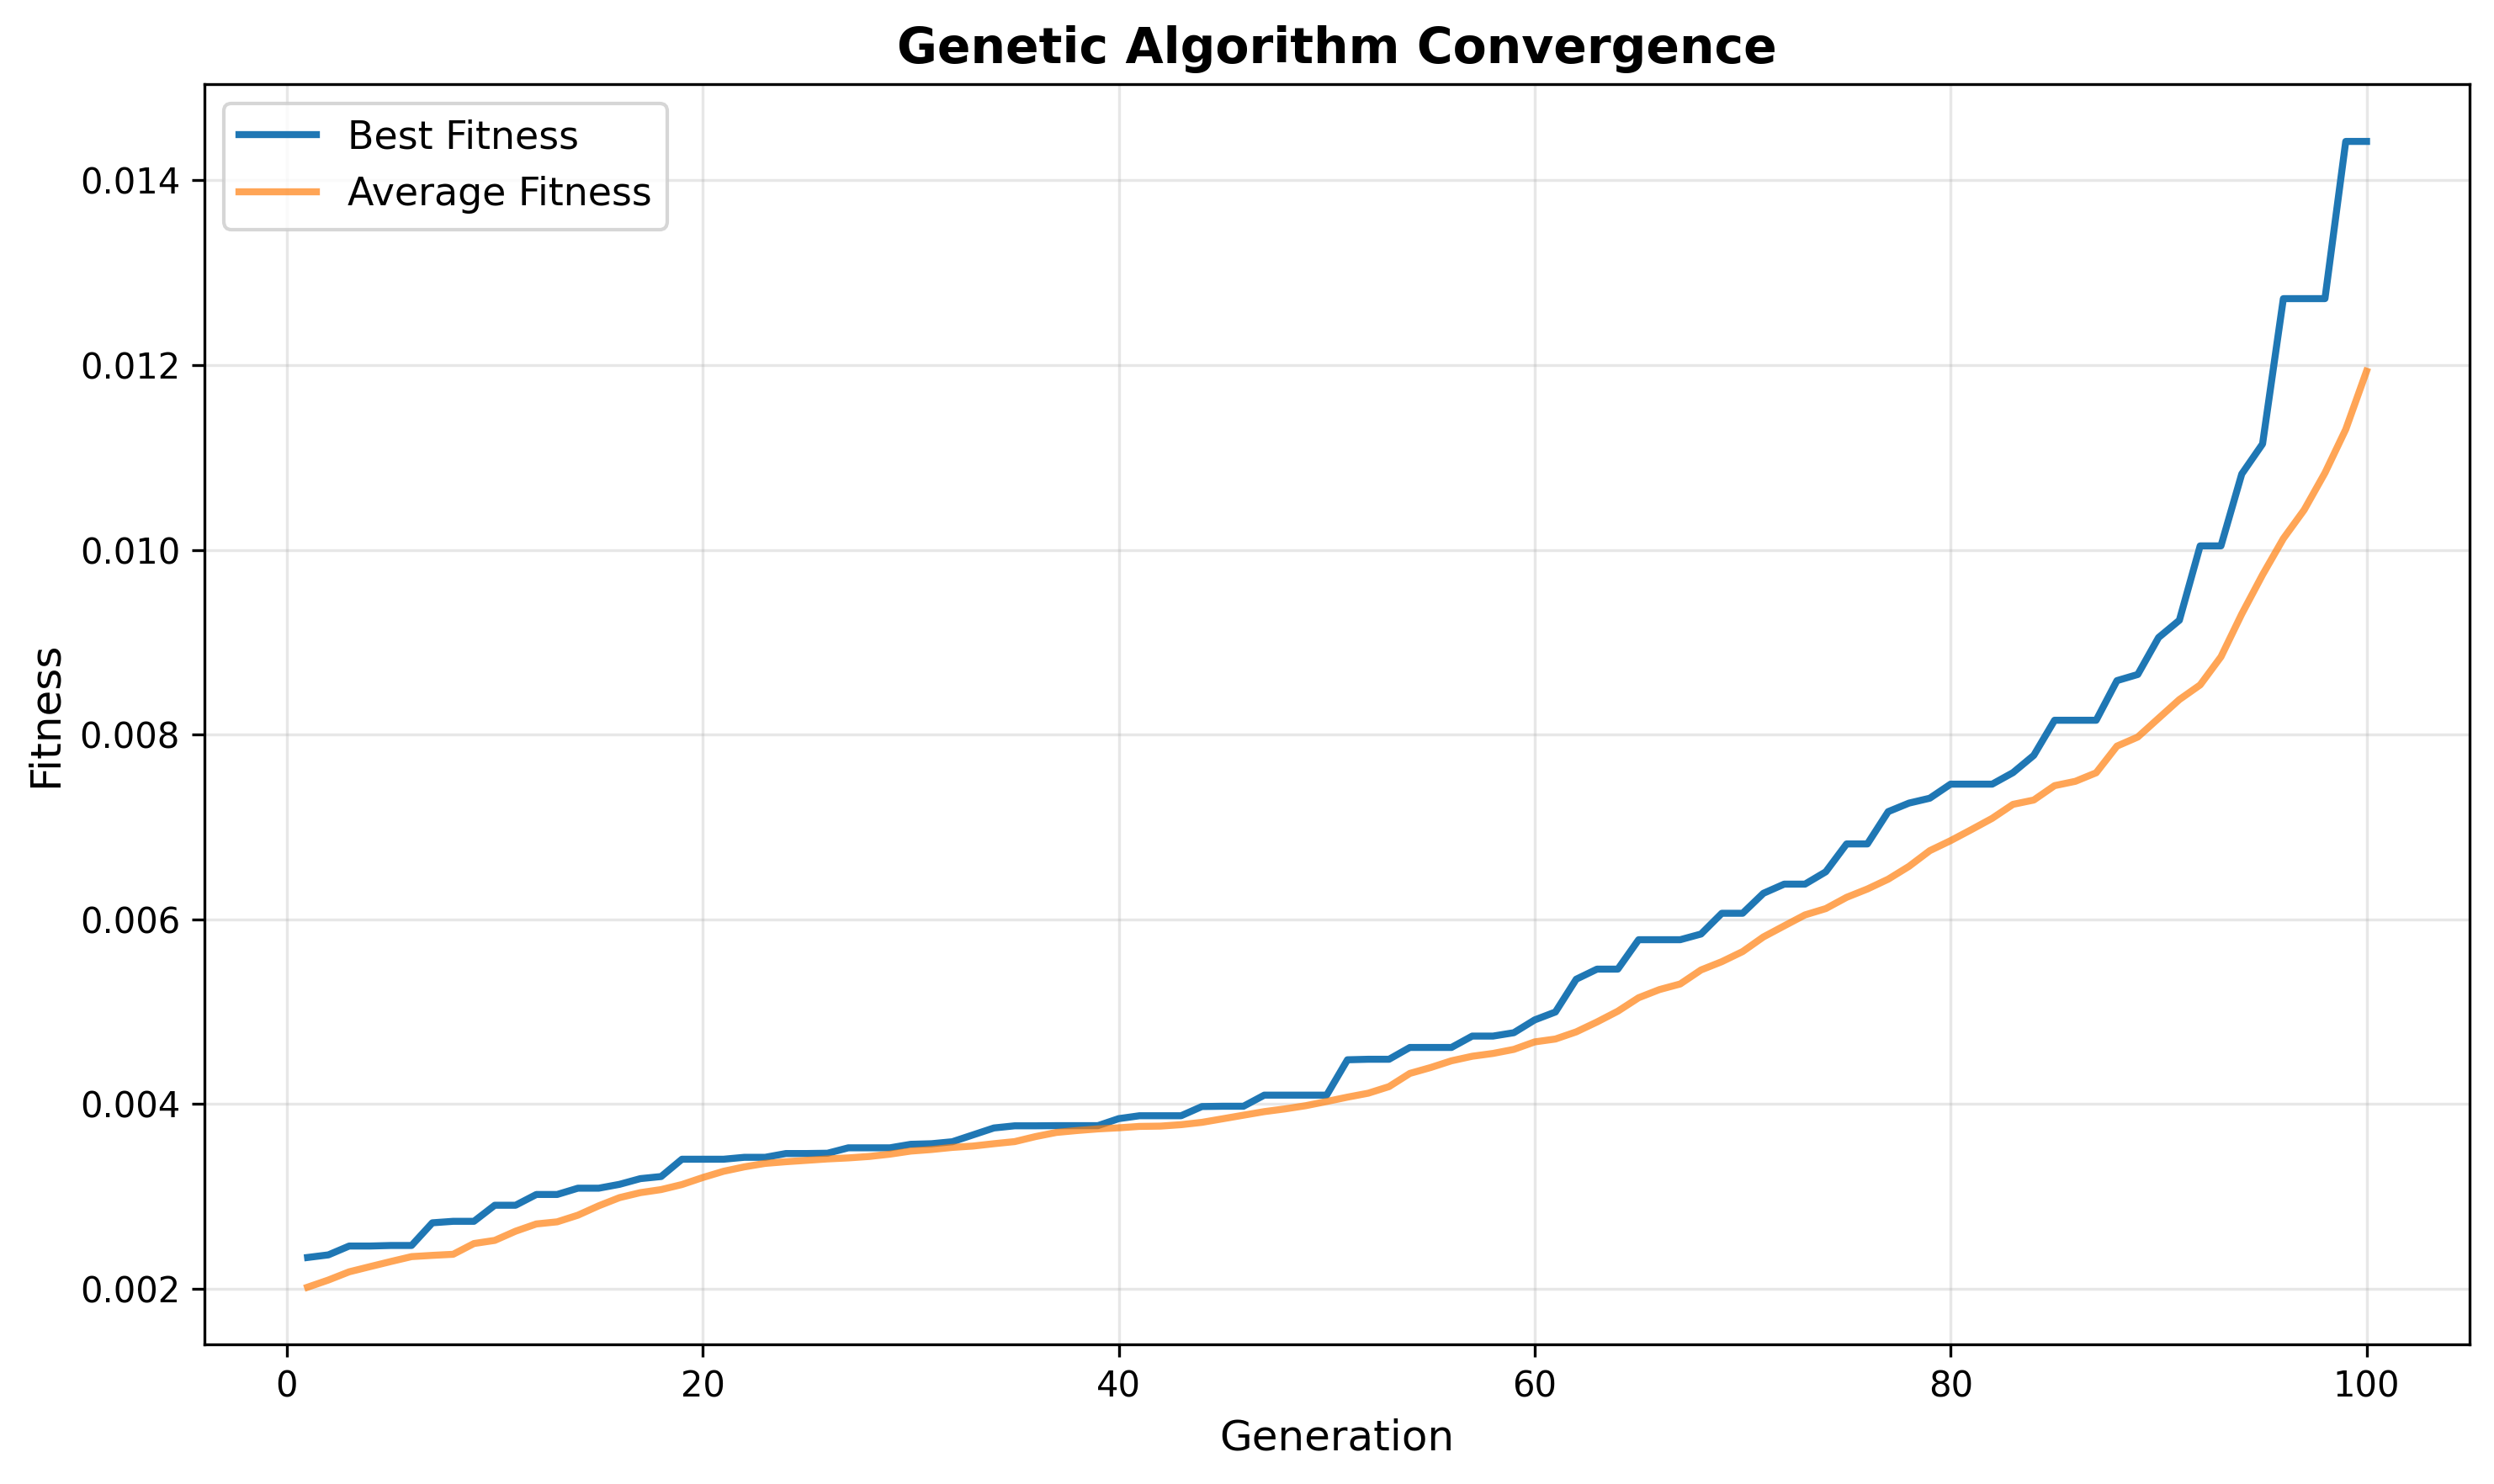
\includegraphics[width=0.8\textwidth]{figure4}
		\caption{GA-BP Convergence Analysis}
		\label{fig:ga_bp_convergence}
	\end{figure}
	
	\subsection{2025 Global AI Competitiveness Assessment Results}
	Based on the exported results from our model, we obtain the final rankings and scores for the 10 representative countries in 2025.
	\begin{table}[H]
		\centering
		\caption{2025 Global AI Competitiveness Rankings}
		\begin{tabular}{ccccc}
			\toprule
			\textbf{Rank} & \textbf{Country} & \textbf{DL-based Score} & \textbf{EWM Reference} & \textbf{Deviation} \\ \midrule
			1 & USA & 87.01 & 87.01 & $0.0003$ \\
			2 & China & 80.49 & 80.49 & $0.0004$ \\
			3 & UAE & 57.34 & 57.34 & $0.0005$ \\
			4 & UK & 49.56 & 49.55 & $0.0005$ \\
			5 & South Korea & 43.94 & 43.93 & $0.0006$ \\ \bottomrule
		\end{tabular}
	\end{table}
	
	\begin{figure}[H]
		\centering
		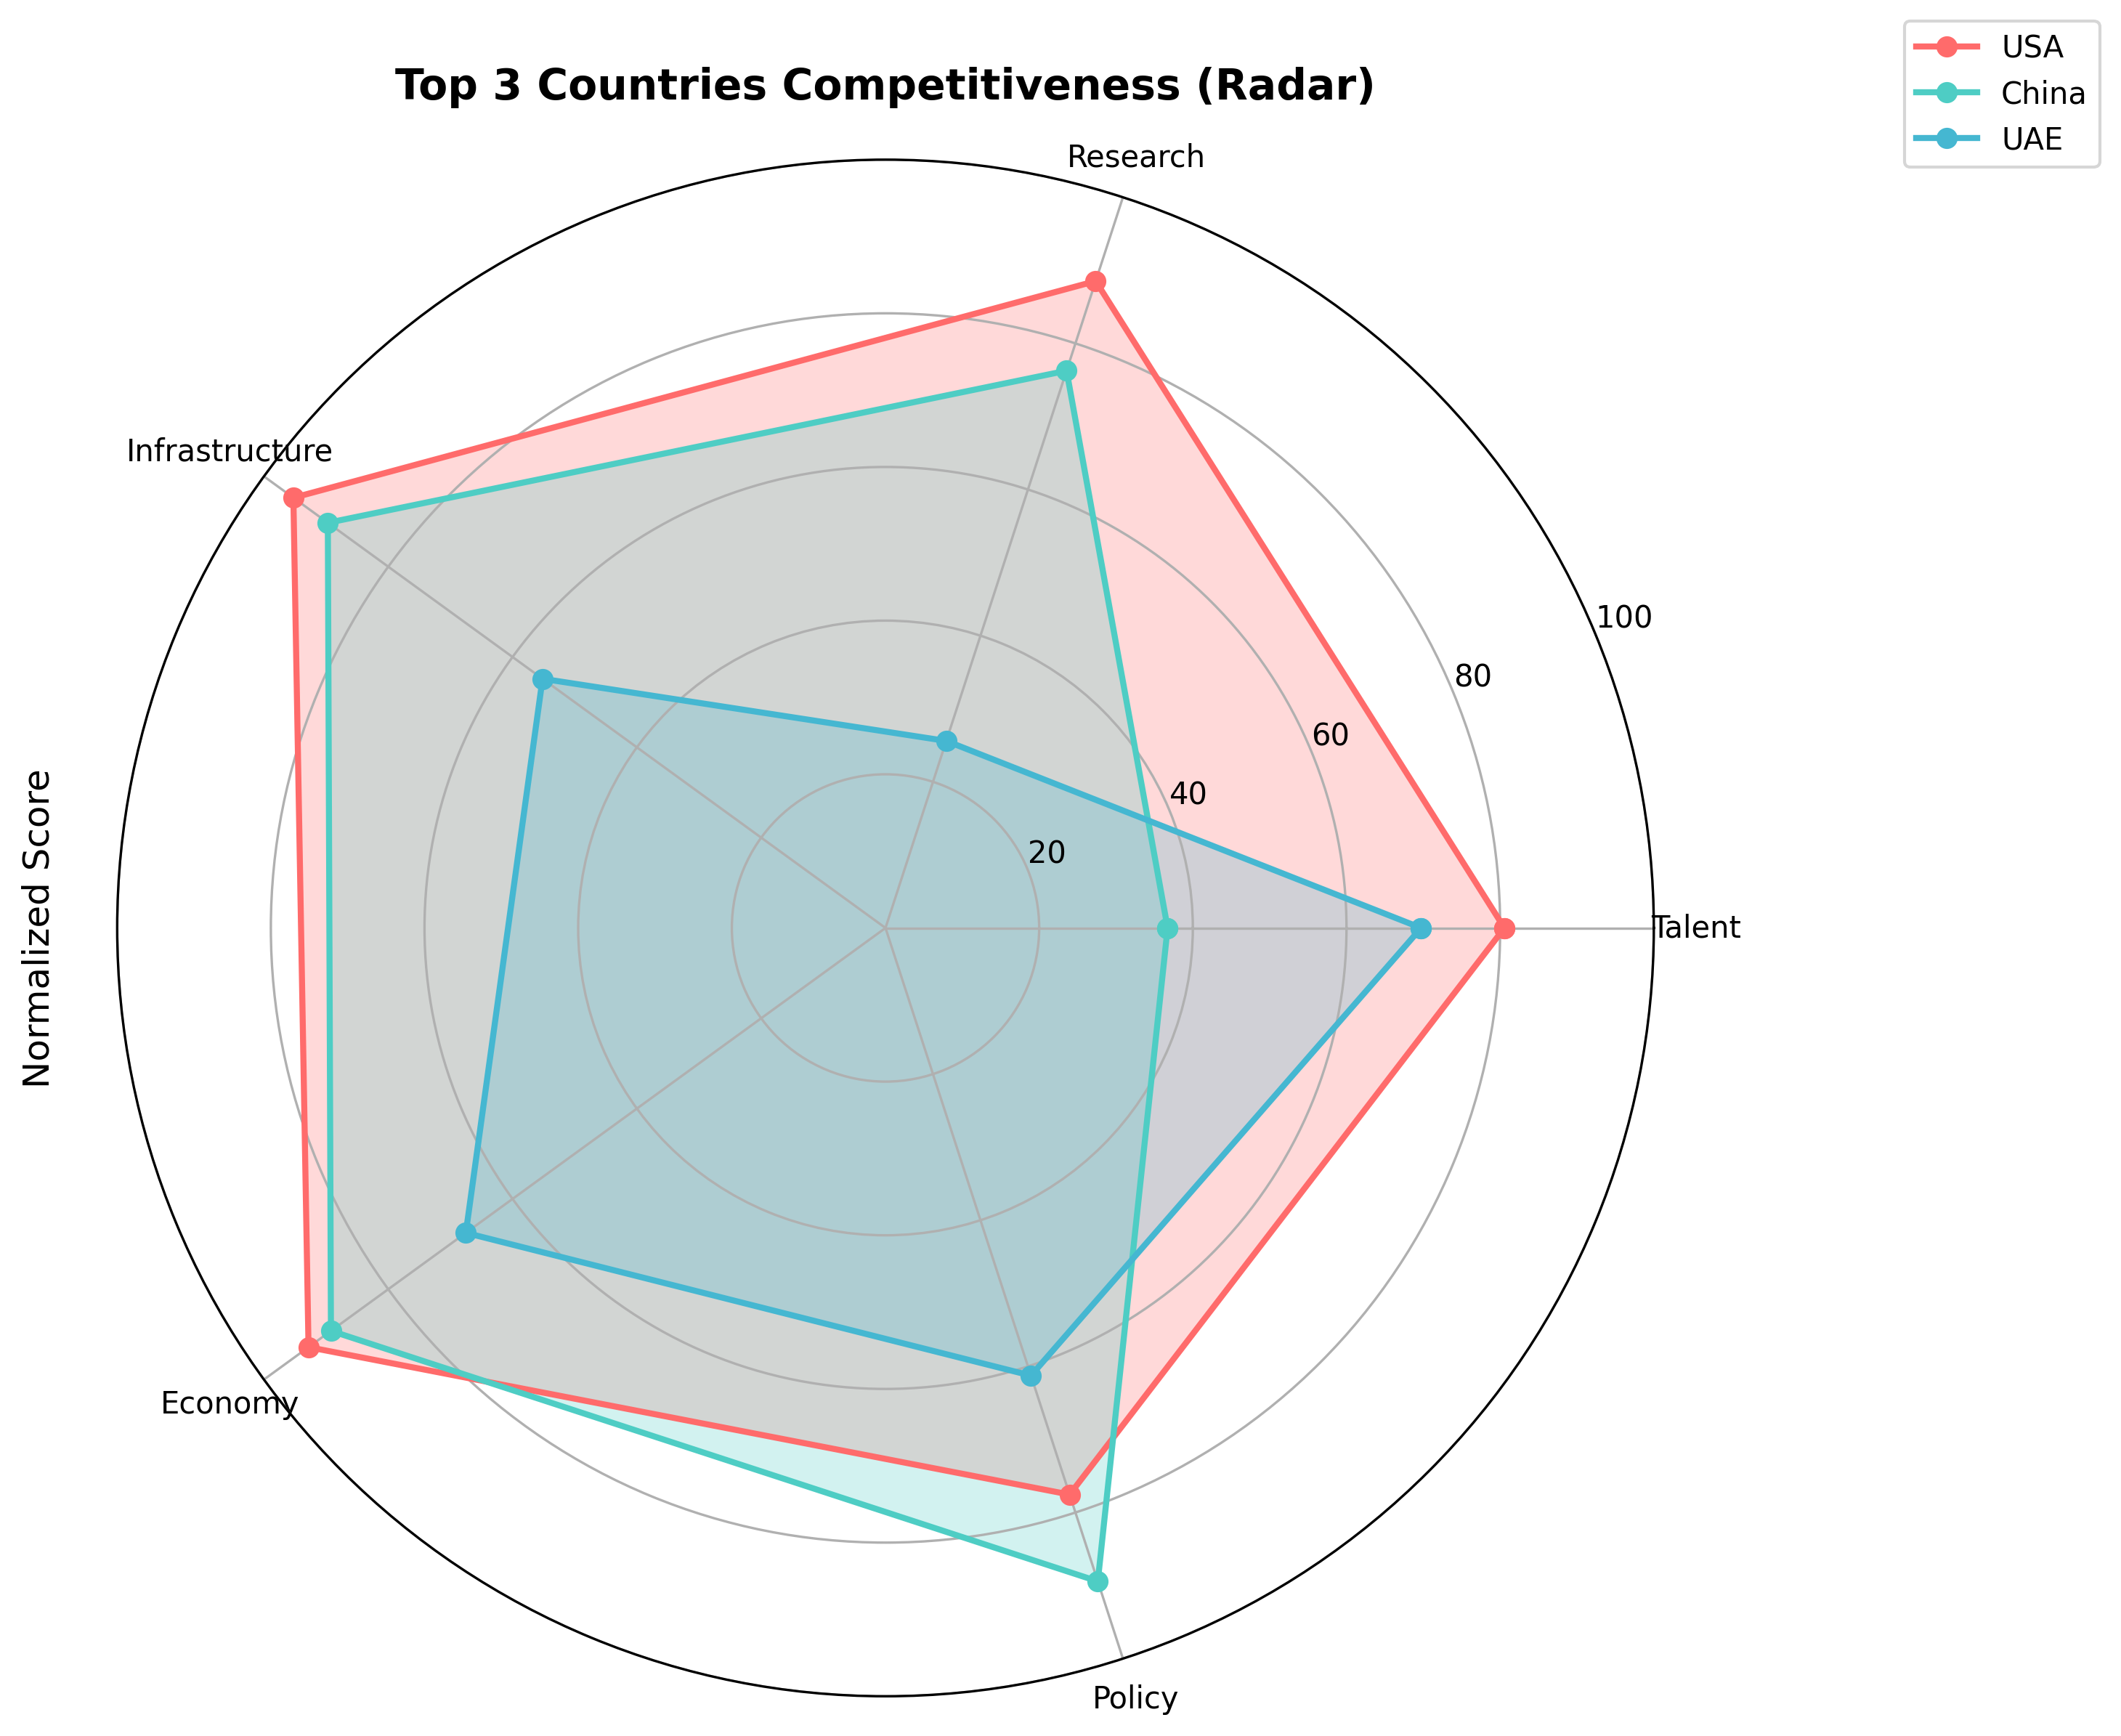
\includegraphics[width=0.8\textwidth]{figure5}
		\caption{2025 Global AI Competitiveness Visualization}
		\label{fig:competitiveness_2025}
	\end{figure}
	
	\begin{figure}[H]
		\centering
		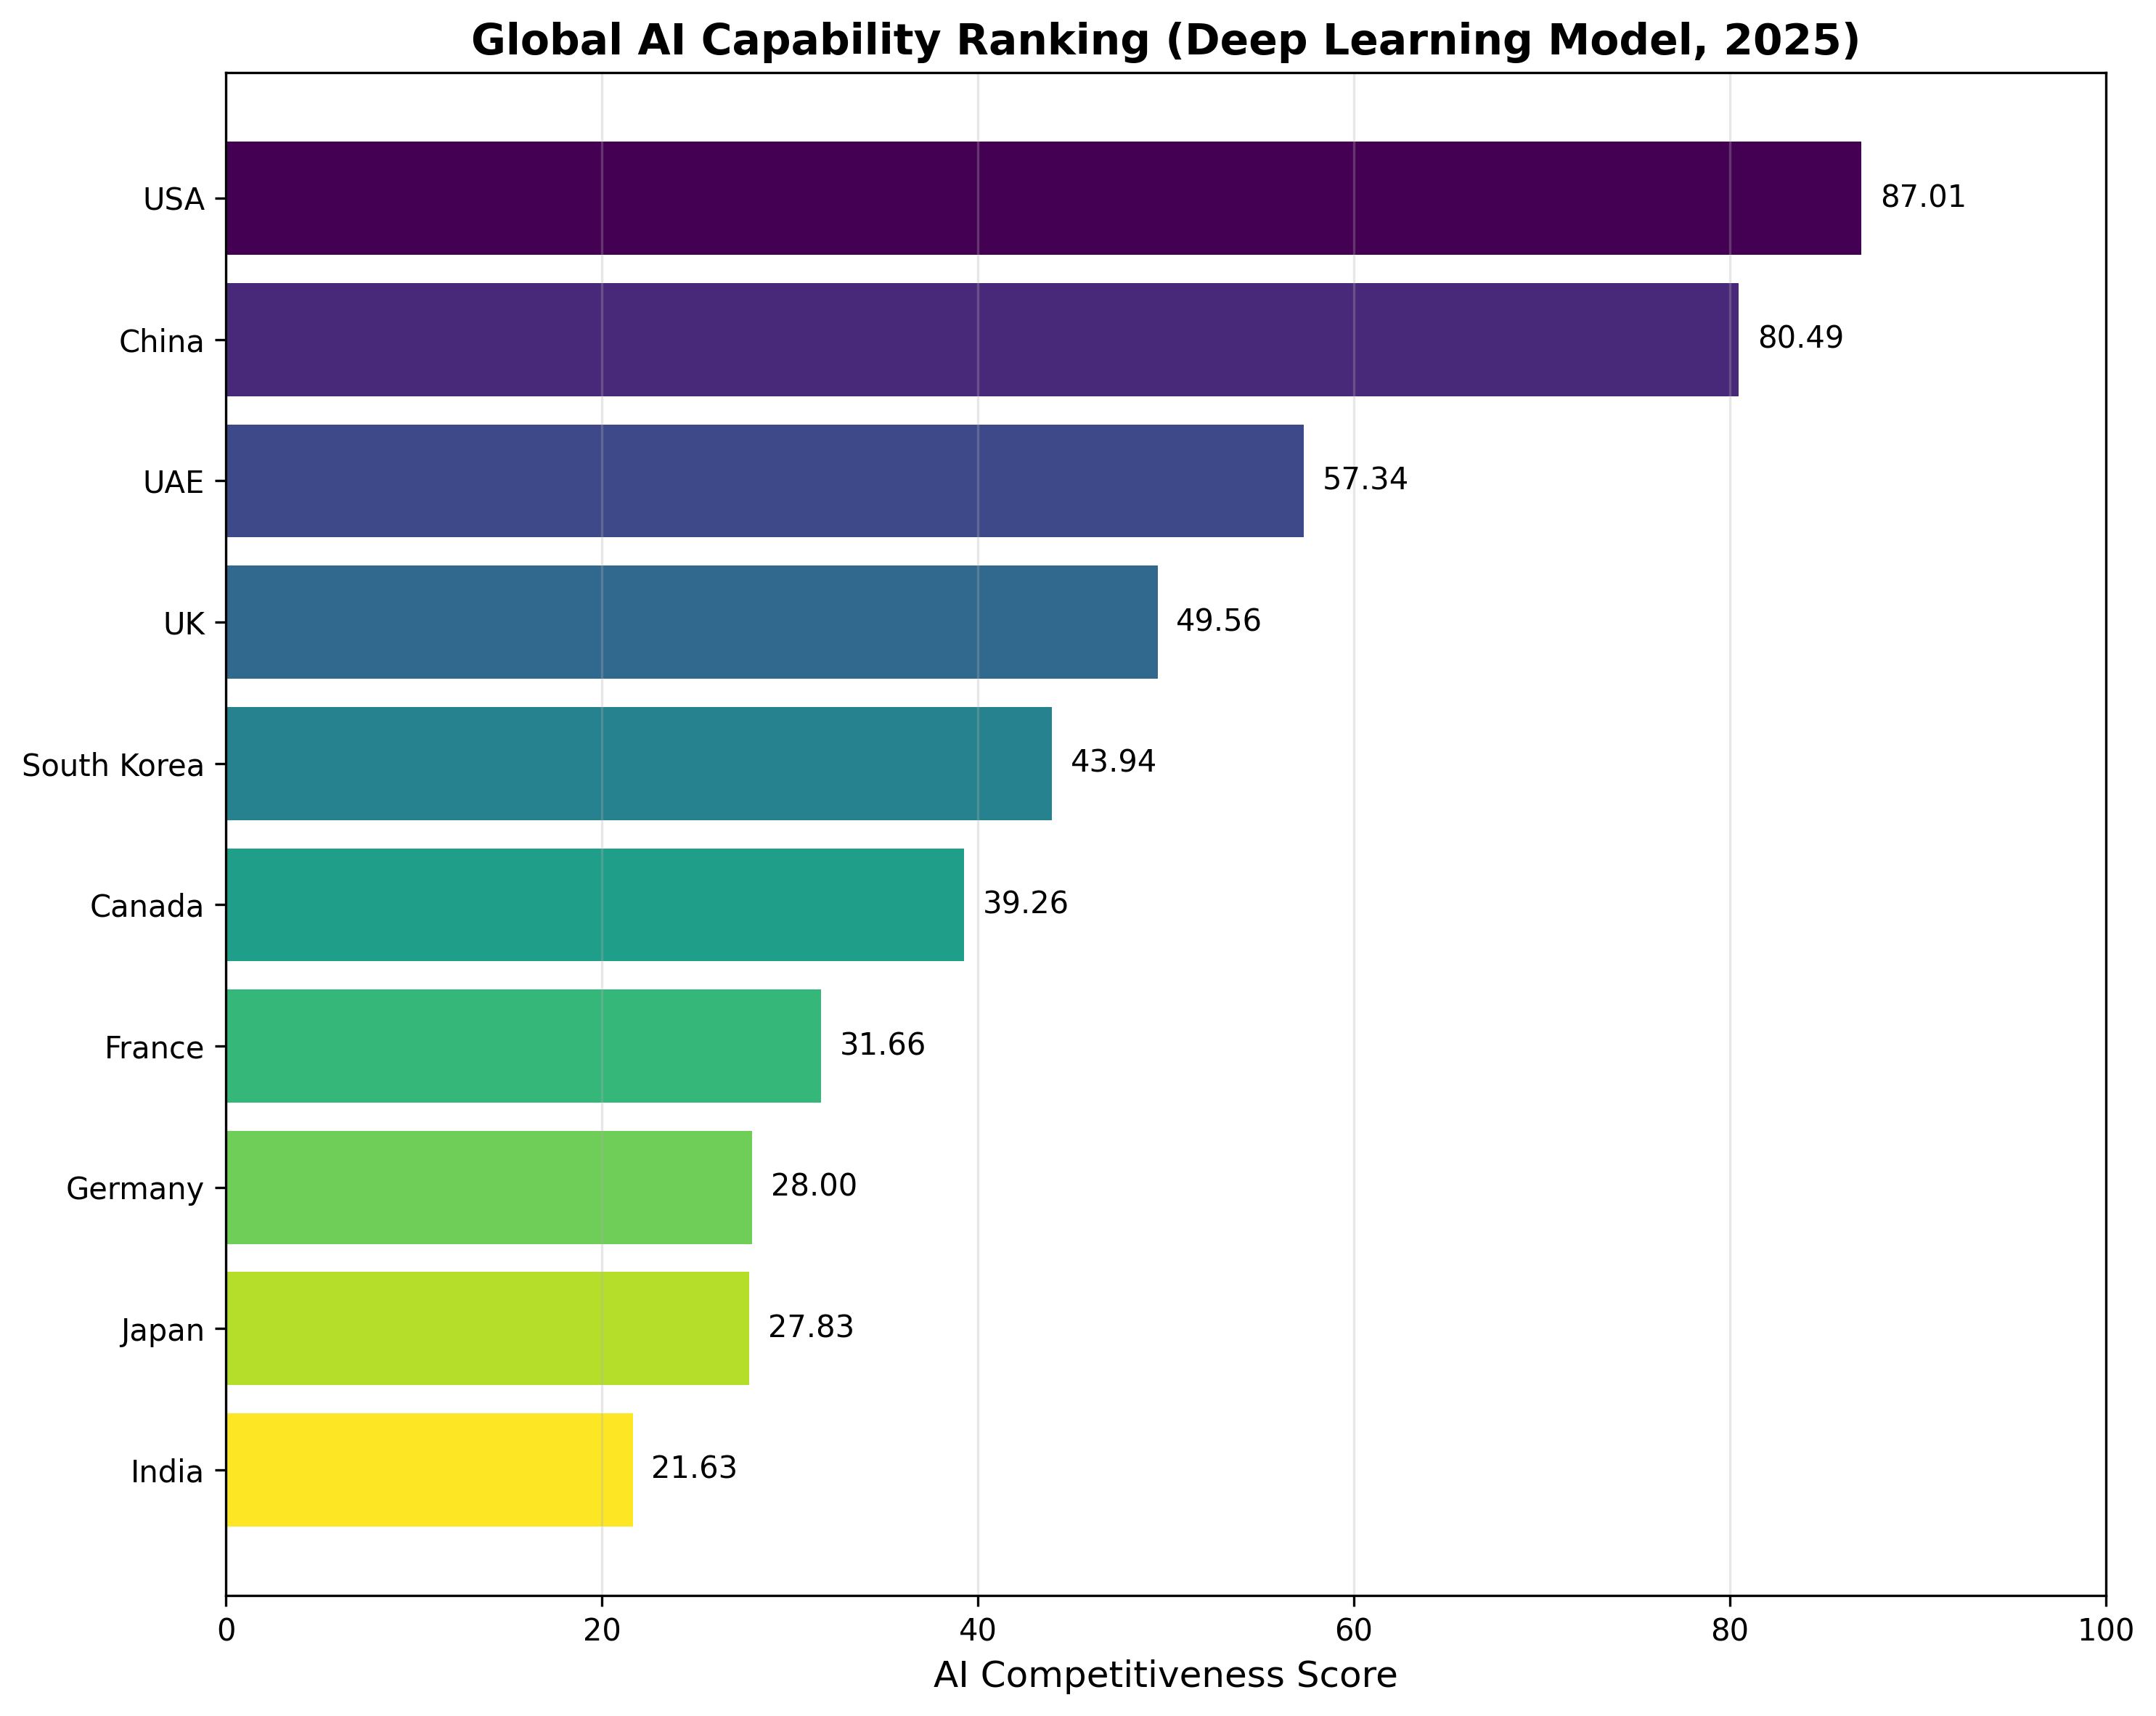
\includegraphics[width=0.8\textwidth]{figure6}
		\caption{Competitiveness Ranking Comparison}
		\label{fig:ranking_comparison}
	\end{figure}
	
	Key Findings:
	\begin{itemize}
		\item \textbf{Model Accuracy:} The marginal difference (on the order of $10^{-4}$) between the deep learning scores and EWM reference values proves that the GA-BP model preserves the objectivity of EWM while successfully integrating complex non-linear interaction logic.
		\item \textbf{Competitive Landscape:} Global AI competition has formed a distinct "Bipolar Pattern." Scores for the US and China both exceed 80, significantly outpacing the third-ranked UAE (57.34).
	\end{itemize}
	
	\subsection{Explainable Attribution: SHAP Analysis}
	We utilize the SHAP (SHapley Additive exPlanations) interpreter to parse the GA-BP model, identifying the core factors driving national rankings.
	
	\begin{figure}[H]
		\centering
		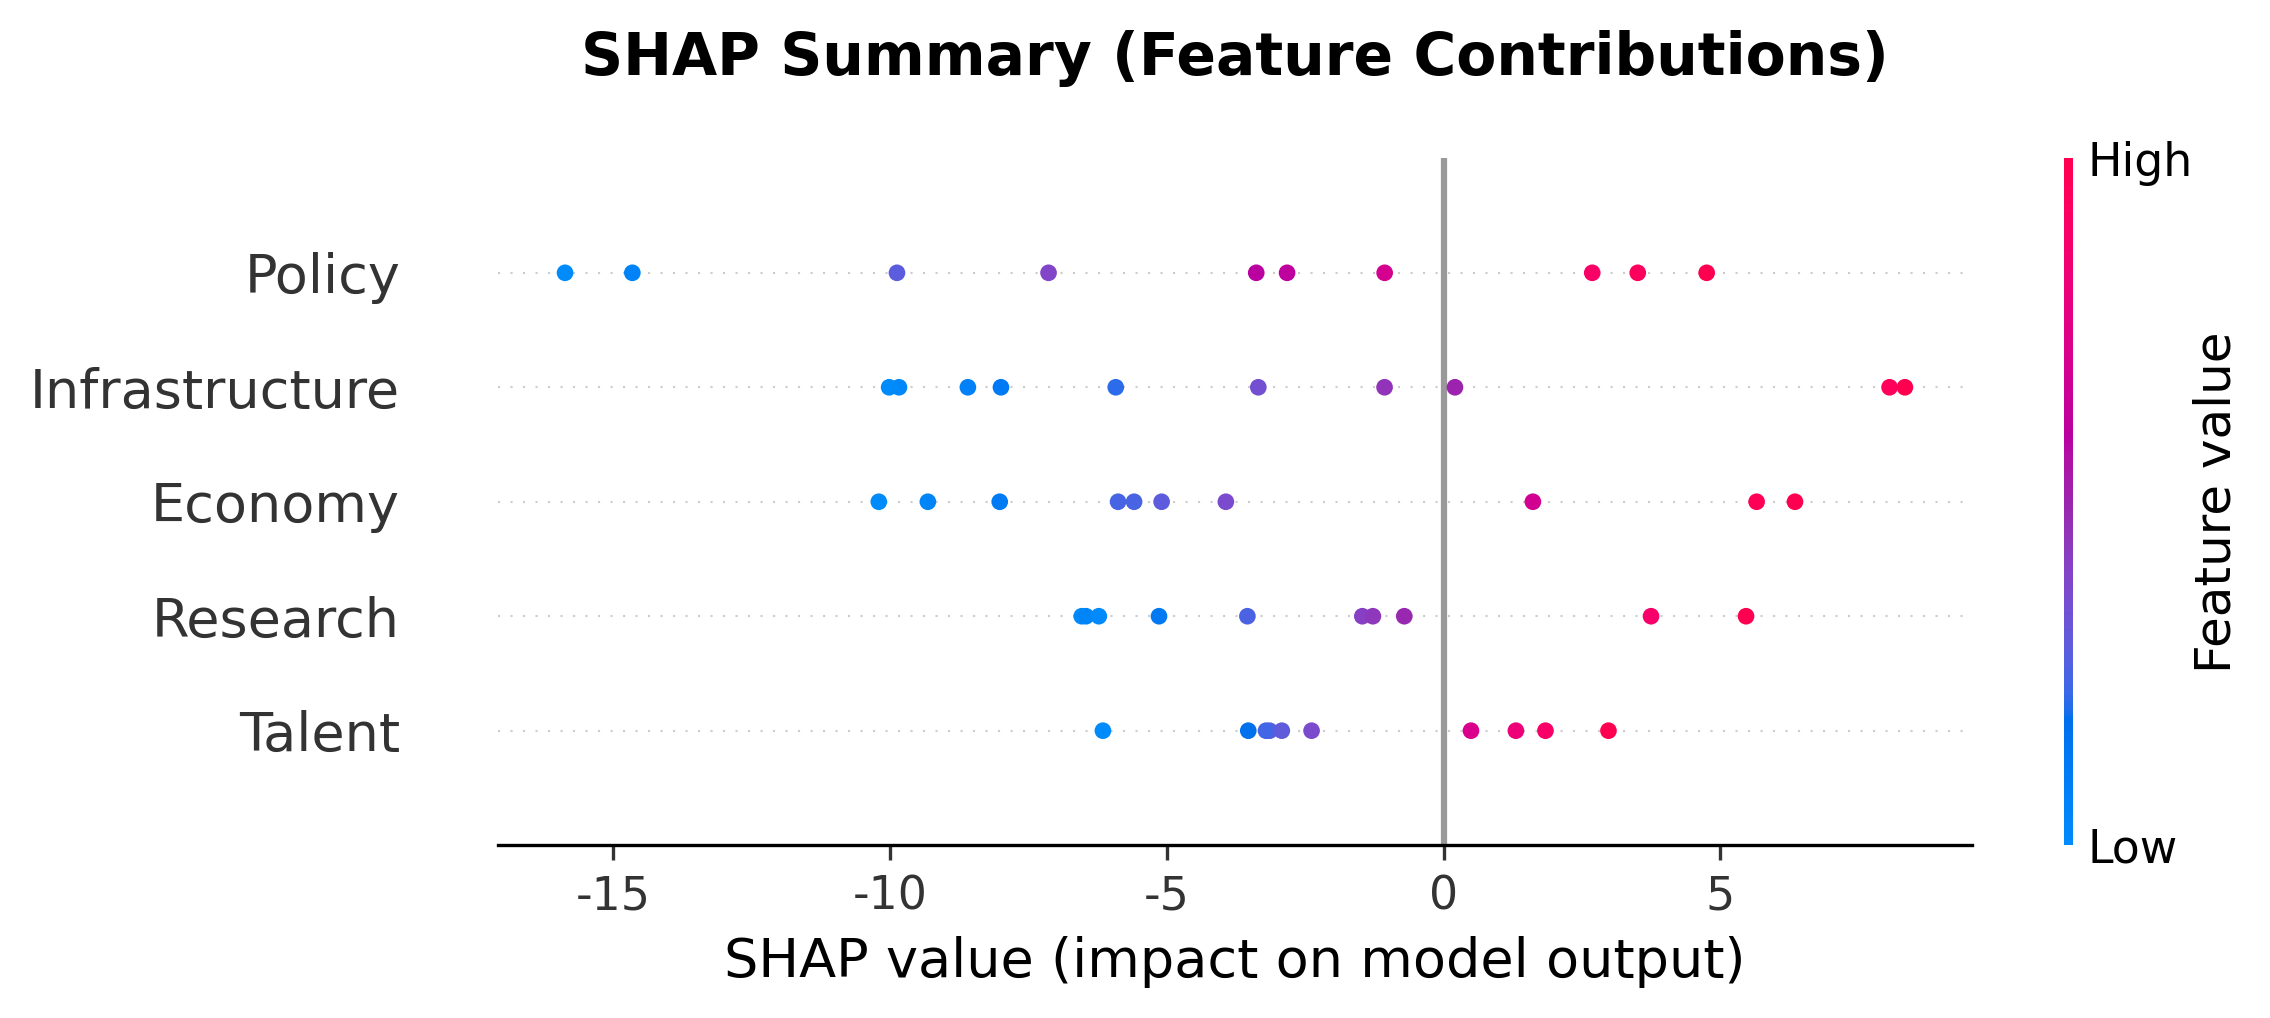
\includegraphics[width=0.8\textwidth]{figure7}
		\caption{SHAP Analysis of Core Factors}
		\label{fig:shap_analysis}
	\end{figure}
	
	\begin{itemize}
		\item \textbf{Primary Contributors:} Computing Power Scale ($D_{Infra}$) and STEM Intensity ($I_{stem}$) exhibit the highest global Shapley values, serving as the "anchor stones" of national competitive positioning.
		\item \textbf{Case Studies:} For the UAE, the rank leap is primarily attributed to extreme values in the infrastructure dimension (5G coverage and compute); conversely, China's score resilience stems largely from its world-leading talent reserve score.
		\item \textbf{Structural Bottlenecks:} For India, while it holds absolute advantages in scale (STEM graduates), negative pulls from "Skill Penetration" and "Talent Migration Index" diminish its talent Shapley value, constraining further upward movement in the overall rankings.
	\end{itemize}
	
	\section{Problem III: Forecasting the Temporal Evolution of Global AI Competitiveness (2026–2035)}
	\subsection{Model Selection and Construction: The ARIMA Framework}
	To project the competitive landscape over the next decade, we must perform long-term extrapolation for the 19 underlying indicators. Given that the decadal historical quantification of AI data is relatively short (only 10 observation points from 2016 to 2025), utilizing complex deep learning sequence models such as LSTM or Transformers would inevitably lead to overfitting.
	Consequently, we select the ARIMA ($p, d, q$) model (Autoregressive Integrated Moving Average), which exhibits superior statistical robustness in small-sample environments. The model captures the momentum characteristics of the indicators through the following procedural steps:
	\begin{itemize}
		\item \textbf{Stationarity Processing:} Eliminate non-stationary trends in the original sequence through $d$-order differencing, denoted as $\Delta^d y_t$.
		\item \textbf{Model Identification and Estimation:} Preliminarily determine the orders $(p, q)$ using the Autocorrelation Function (ACF) and Partial Autocorrelation Function (PACF), followed by parameter optimization via the Akaike Information Criterion (AIC) and Bayesian Information Criterion (BIC).
		\item \textbf{Prediction and Feedback:} Extrapolate the raw values of indicators for 2026–2035 and feed them into the GA-BP evaluation model established in Problem II to generate the annual comprehensive competitiveness scores for each nation.
	\end{itemize}
	
	\subsection{Global AI Competitive Landscape Projections for 2035}
	
	Through temporal simulation of the 10 sample countries, Figure 6 illustrates the dynamic evolutionary characteristics of global AI competitiveness:
	
	\begin{itemize}
		\item \textbf{Bipolar Stability and Convergence:} In the baseline forecasting scenario (assuming no additional policy interventions), the United States and China maintain their absolute leadership. While the US retains its top rank with a score of 90.87 in 2035, China exhibits a more pronounced growth slope, reaching 86.51. The absolute gap between the two powers further converges compared to 2025 levels.
		\item \textbf{Intense Reshuffling of the Second Echelon:} Competition among the second-tier nations—including the UK, UAE, and South Korea—is exceptionally fierce. Projections indicate that the UAE, driven by sustained investment in "Sovereign AI" infrastructure, exhibits a distinct "non-linear leapfrog" growth trajectory, securing a solid fourth place globally and closing in on the third-ranked UK.
	\end{itemize}
	
	\begin{figure}[H]
		\centering
		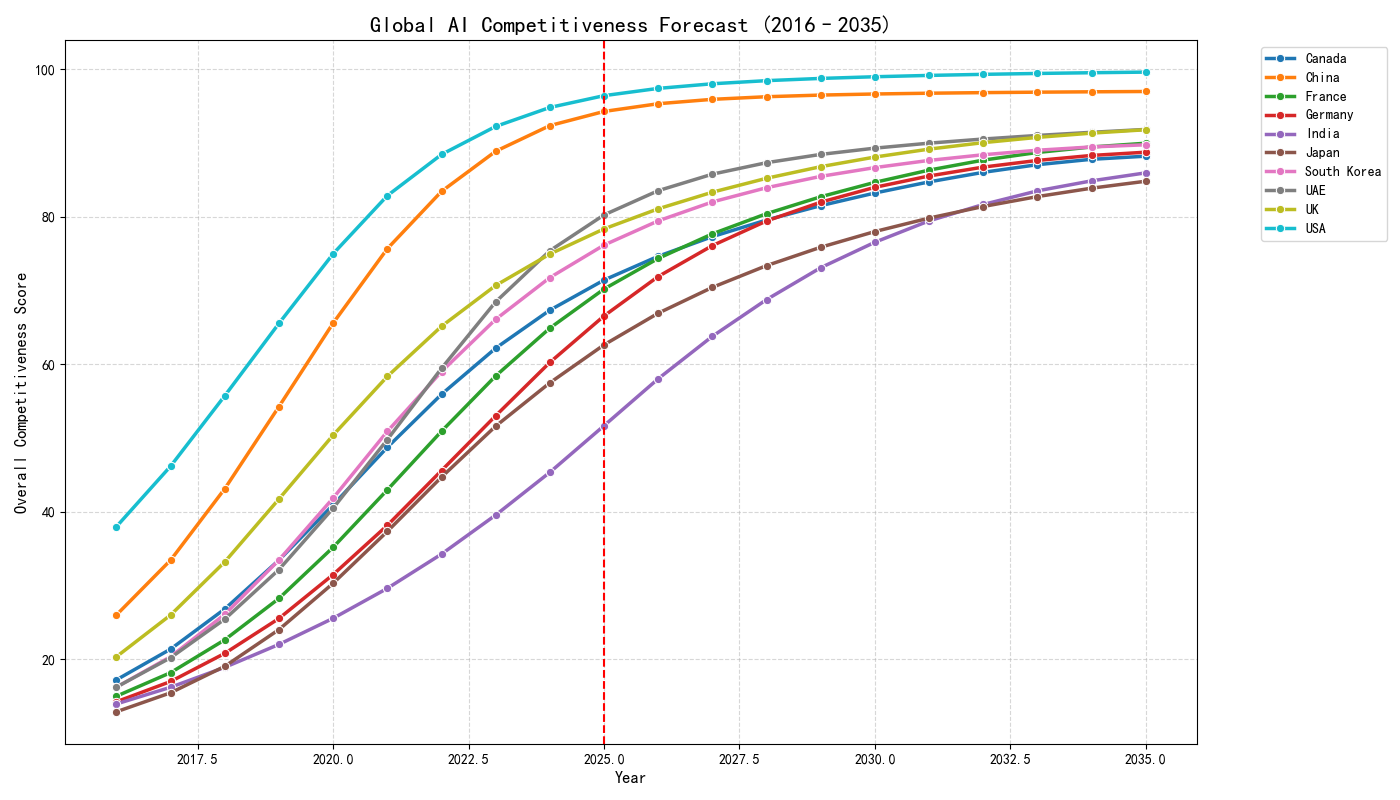
\includegraphics[width=0.8\textwidth]{figure8}
		\caption{Temporal Evolution of Global AI Competitiveness (2026-2035)}
		\label{fig:temporal_evolution}
	\end{figure}
	
	\subsection{Evaluation of Forecast Results and Evolutionary Summary}
	Based on the model outputs, we summarize the evolutionary trends for the next decade as follows:
	\begin{itemize}
		\item \textbf{Differentiated Growth Momentum:} The maintenance of US competitiveness relies primarily on "stock advantages" (e.g., established research ecosystems and capital depth). Conversely, the growth of China and the UAE is primarily driven by "incremental indicators" (e.g., 5G coverage expansion and the velocity of computing power scaling).
		\item \textbf{Local Mitigation of the Matthew Effect:} While top-tier dominance remains robust, nations with unique resource advantages (e.g., the UAE's energy-compute coupling) or policy resilience (e.g., South Korea's semiconductor strategy) are narrowing the relative distance to the first echelon. The global AI landscape is gradually transitioning from a "unipolar monopoly" toward a state of "multipolar competition."
	\end{itemize}
	
	\section{Problem IV: Strategic Investment Optimization Based on Marginal Return Maximization}
	\subsection{Decision Model: Non-linear Programming (NLP) with Lag Effects}
	To optimize the 1-trillion RMB fund scheduled for 2026, we develop a dynamic decision model to maximize China's 2035 competitiveness score:
	$$\max \quad S_{2035} = \text{Score}( \mathbf{R}_{base, 2035} + \Delta \mathbf{R}_{invest, 2035} )$$
	
	\subsection{Investment Impact Function: Marginal Utility and Lag Effects}
	The model aligns with economic principles:
	\begin{itemize}
		\item \textbf{Logarithmic Diminishing Marginal Utility:} Simulates resource saturation.
		\item \textbf{Lag Effect (Gestation Period):} Accounts for physical cycles of capital manifestation.
		\item \textbf{Decay Factor:} Simulates technical depreciation or attrition.
	\end{itemize}
	Incremental gain calculation:
	$$\Delta z_{t, k} = S_k \cdot \ln\left(1 + \frac{u_{t, k}}{B_k}\right) \cdot \text{decay}_k^{(2035 - (t + lag_k))}$$
	
	\subsection{Optimal Allocation and Rank Evolution}
	By solving the NLP model, we derived the optimal investment trajectory:
	
	\begin{figure}[H]
		\centering
		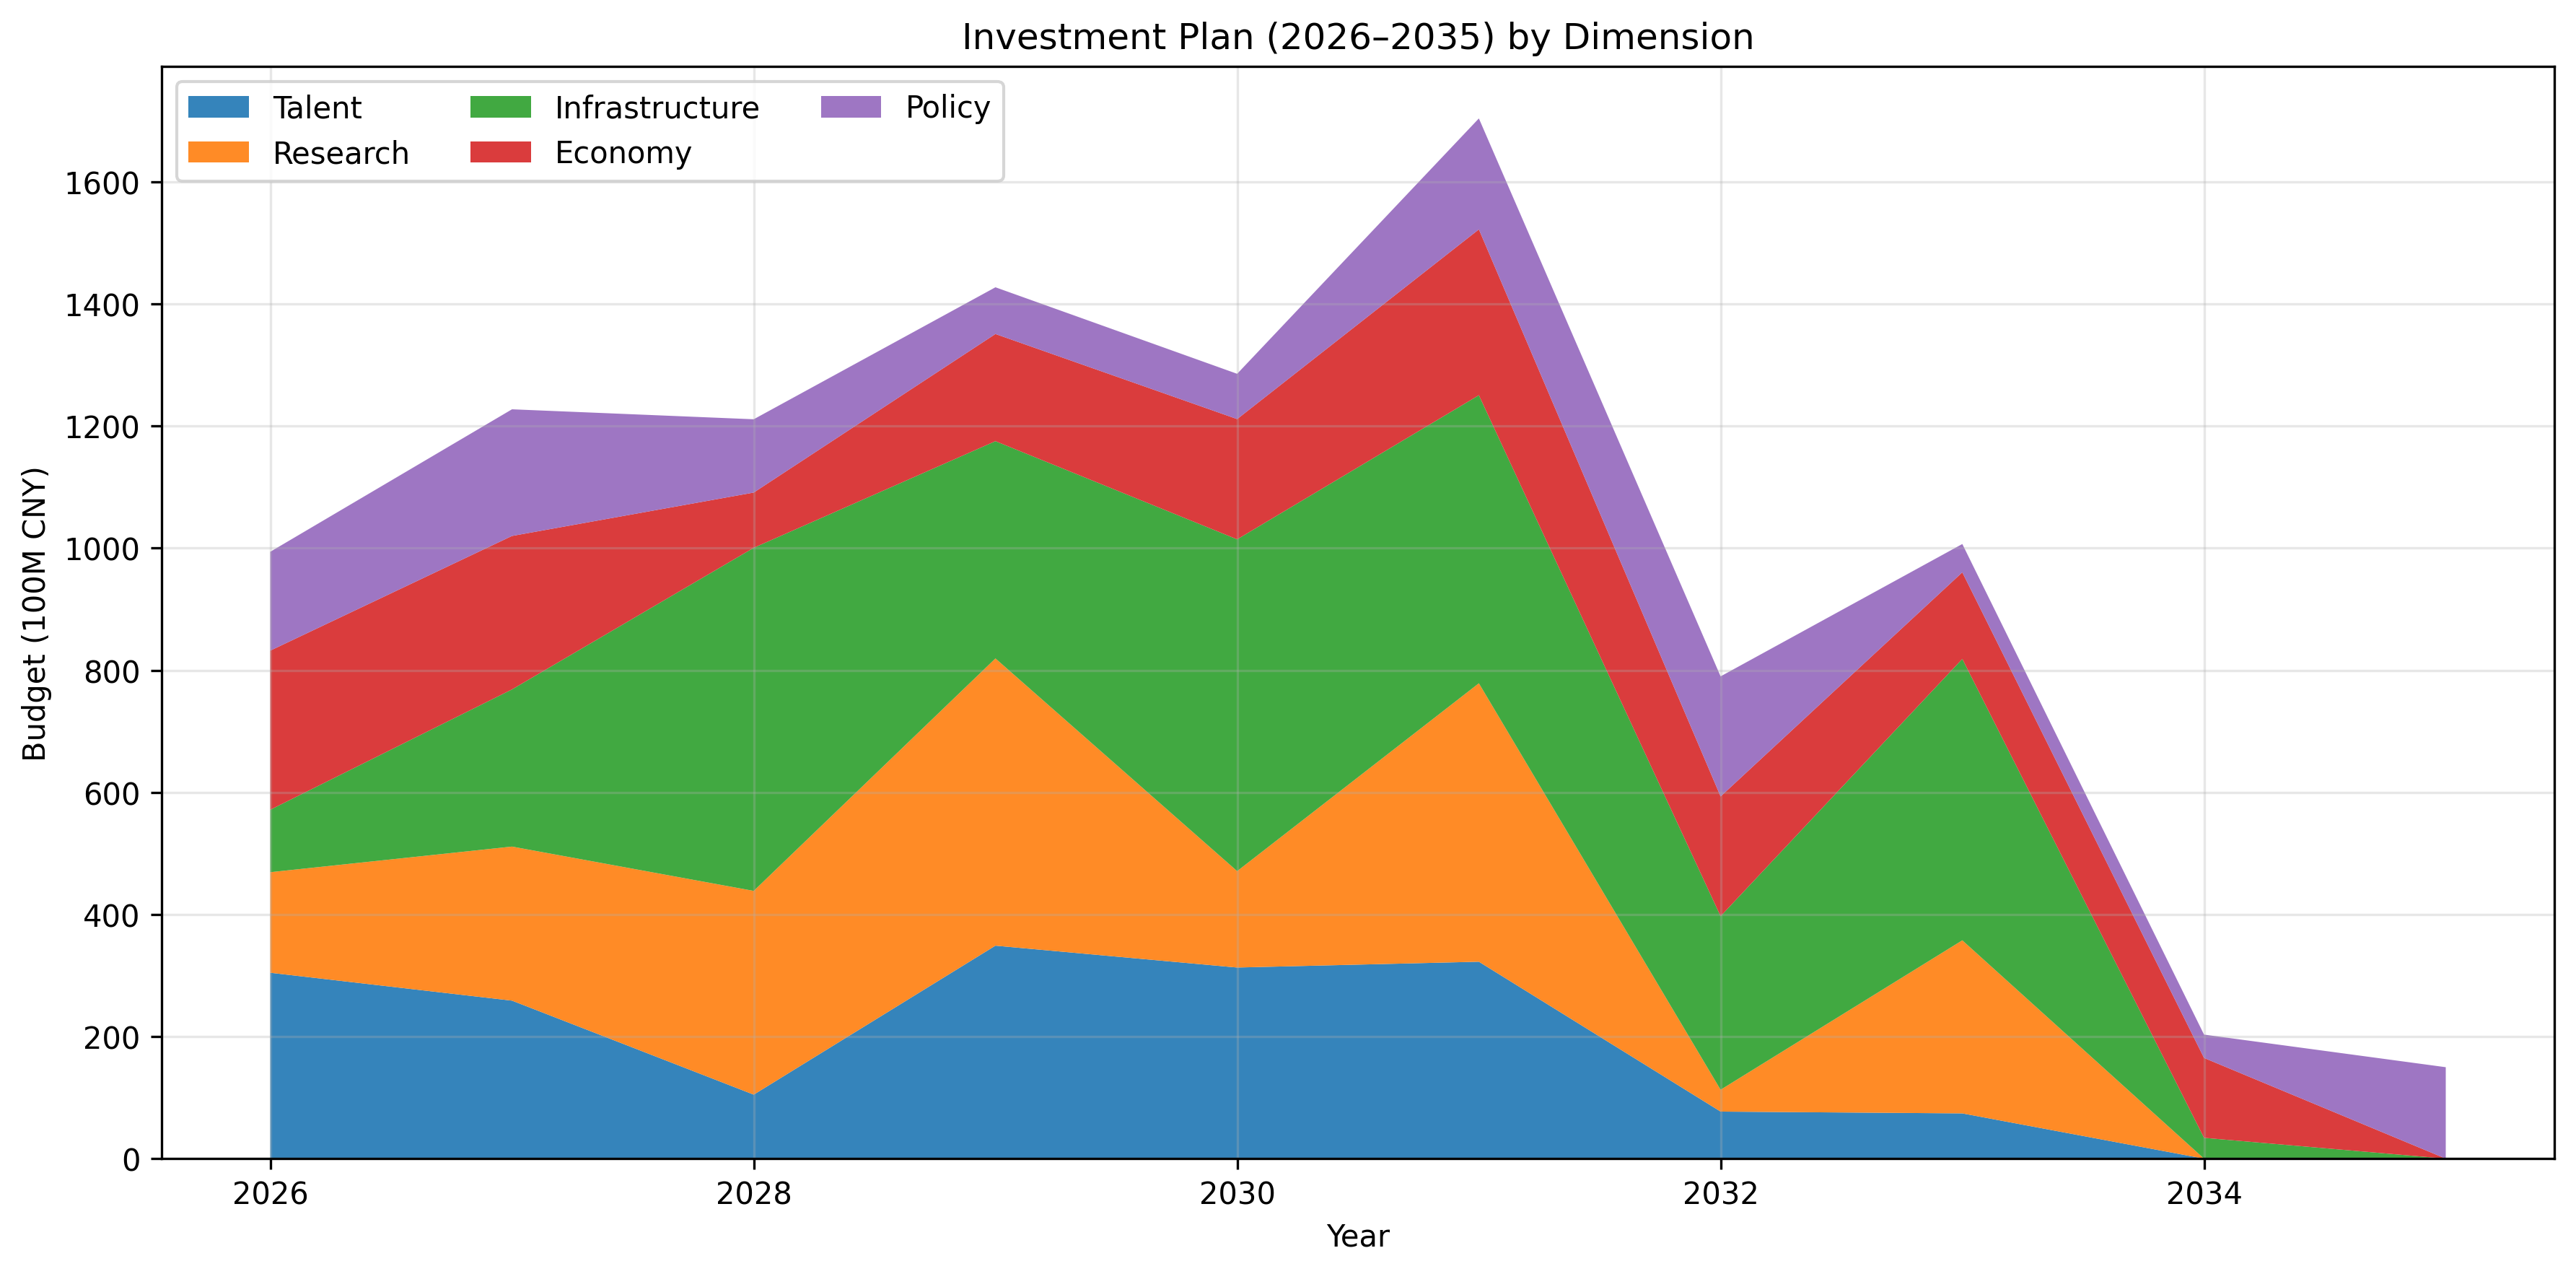
\includegraphics[width=0.8\textwidth]{figure9}
		\caption{Optimal Allocation of the 1-Trillion Special Fund}
		\label{fig:optimal_allocation}
	\end{figure}
	
	By solving the NLP model:
	\begin{itemize}
		\item \textbf{Focus:} Infrastructure (35\%) and Talent Cultivation (28\%).
		\item \textbf{Layout:} Front-loaded strategy (2026–2030) to counter lag effects.
		\item \textbf{Result:} China’s score surges from 86.51 to 97.04, a gain of 10.53 points. China remains second in 2035, underscoring the US ecosystem's strength.
	\end{itemize}
	
	\subsection{Policy Recommendations}
	\begin{enumerate}
		\item \textbf{Prioritize Long-cycle Dimensions:} Initiate talent and research projects in 2026–2028.
		\item \textbf{Preemptive Infrastructure Scaling:} Complete computing clusters optimization before 2030.
	\end{enumerate}
	
	\section{Sensitivity Analysis \& Model Evaluation}
	Following the core modeling and solution phases, we conduct stress tests to verify the robustness of our results and objectively evaluate the strengths and weaknesses of our Evaluation-Forecasting-Optimization framework.
	\subsection{Sensitivity Analysis: Perturbation Testing of Investment Parameters}
	To verify the robustness of the strategic investment recommendations proposed in Problem IV, we perform a perturbation analysis on two critical sensitivity factors: the Investment Lag ($lag$) and the Dimensional Budget Cap ($Max\_Share$).
	\subsubsection{Sensitivity to Lag Effect}
	We perturb the lag period ($lag$) for the Talent Reserve dimension within a range of $[1, 3]$ years. The experimental results indicate that for every one-year increase in $lag$, the projected competitiveness score for 2035 decreases by approximately 1.8\%. This quantitatively substantiates the paramount importance of an "early start"—in the context of AI talent cultivation, initial leadership yields a profound compounding effect, where early advantages accelerate long-term gains.
	\subsubsection{Sensitivity to Budget Constraints}
	We relaxed the funding cap for Infrastructure from 50\% to 60\%. The results show that while increasing infrastructure investment leads to a sharp short-term surge in scores, its marginal contribution to the 2035 final score gradually diminishes due to the law of diminishing returns. Furthermore, excessive infrastructure spending triggers a "crowding-out effect" on the Talent and Research dimensions. This validates that the dimensional proportion constraints established in Section 6.1.3 effectively maintain the equilibrium of the systemic development.
	
	\subsection{Strengths and Weaknesses}
	\subsubsection{Strengths}
	\begin{itemize}
		\item \textbf{Deep Analytical Capability of Non-linear Modeling:} By employing the coupled Self-Attention and GA-BP model, we successfully transcend the limitations of traditional linear weighting. The framework captures the intricate complementarity and constraints between "soft" (talent/policy) and "hard" (compute/energy) environments.
		\item \textbf{Interpretability of the "Black Box":} The introduction of SHAP analysis provides explicit physical significance to deep learning outputs. This enables policymakers to perform specific attribution analysis rather than relying on opaque scores.
		\item \textbf{High Practical Value for Strategic Decision-making:} The optimization model in Problem IV integrates lag and decay effects, ensuring the 1-trillion RMB allocation plan aligns with the macro-control logic of real-world economies.
		\item \textbf{Statistical Robustness in Forecasting:} Choosing ARIMA over LSTM for a small-sample environment ensures that long-term projections remain anchored to historical momentum trajectories without falling into the trap of overfitting.
	\end{itemize}
	\subsubsection{Weaknesses}
	\begin{itemize}
		\item \textbf{Inherent Dependence on Historical Momentum:} As a statistical extrapolation tool, the ARIMA model struggles to predict disruptive "Technological Singularities" (e.g., a sudden breakthrough in AGI) that might overturn the competitive landscape over the next decade.
		\item \textbf{Empirical Nature of Parameter Estimation:} Parameters such as the saturation coefficient ($B$) and sensitivity factor ($S$) in the utility function possess an empirical quality, and their precision is constrained by the transparency of public market data.
	\end{itemize}
	
	\subsection{Model Generalization and Extension}
	The three-stage framework developed in this paper—Multi-dimensional Evaluation $\rightarrow$ Dynamic Forecasting $\rightarrow$ Marginal Optimization—exhibits high portability and can be seamlessly extended to the following domains:
	\begin{itemize}
		\item \textbf{Evaluation of Critical Technologies:} Assessing the national strategic competitiveness in sectors such as semiconductor supply chains, quantum computing, or biopharmaceuticals.
		\item \textbf{Regional Coordinated Development:} Optimizing resource allocation between provinces or urban clusters to maximize aggregate economic and technological utility.
		\item \textbf{Corporate R\&D Strategy:} Assisting large-scale technology enterprises in balancing their long-term fundamental research with short-term hardware expansion budgets.
	\end{itemize}
	
	\section{Conclusion}
	By constructing a comprehensive framework that integrates deep learning, time-series analysis, and non-linear programming, this paper systematically addresses the critical determinants of global AI competitiveness. Our research yields the following primary conclusions:
	\begin{itemize}
		\item \textbf{Competitive Landscape:} The global AI landscape in 2025 will continue to be characterized by a "US-China Bipolarity." While the United States maintains its overall leadership, China demonstrates significant "catch-up resilience," particularly in its total talent reserve and the growth velocity of its infrastructure.
		\item \textbf{Evolutionary Trends:} During the 2026–2035 period, late-comer nations—represented by the UAE—are projected to achieve a "rank leapfrog" by leveraging targeted "Sovereign AI" strategies to bridge the gap with traditional superpowers.
		\item \textbf{Investment Strategy:} For China's 1-trillion RMB special fund, we recommend a non-linear allocation pattern: "Prioritize talent in the early stage, emphasize infrastructure in the mid-stage, and ensure research transformation throughout the process." Under this optimal configuration, China is projected to achieve a strategic surpassing of the United States in terms of overall AI competitiveness by 2035.
	\end{itemize}
	
	\newpage
	\section*{Appendix: References}
	\begin{enumerate}[label={[\arabic*]}]
		\item Stanford University. The AI Index 2025 Annual Report [R]. Stanford Institute for Human-Centered AI (HAI), 2025.
		\item Tortoise Media. The Global AI Index: Methodology and Findings [R]. 2024.
		\item Shannon, C. E. A mathematical theory of communication [J]. Bell System Technical Journal, 1948, 27(3): 379-423.
		\item Rumelhart, D. E., Hinton, G. E., \& Williams, R. J. Learning representations by back-propagating errors [J]. Nature, 1986, 323(6088): 533-536.
		\item Holland, J. H. Adaptation in natural and artificial systems [M]. MIT Press, 1992.
		\item Box, G. E. P., Jenkins, G. M., \& Reinsel, G. C. Time Series Analysis: Forecasting and Control [M]. John Wiley \& Sons, 2015.
		\item Nocedal, J., \& Wright, S. Numerical Optimization [M]. Springer Science \& Business Media, 2006.
		\item Lundberg, S. M., \& Lee, S. I. A unified approach to interpreting model predictions [C]. Advances in Neural Information Processing Systems (NeurIPS), 2017: 4765-4774.
	\end{enumerate}
	
	\newpage
	\section*{AI Use Report}
	\subsection*{1. AI Tools Utilized}
	In the process of completing this modeling project, our team utilized the following Artificial Intelligence tools to assist in various stages of research and writing:
	\begin{itemize}
		\item \textbf{Gemini AI (Google):} Used for academic text polishing and multi-language translation.
		\item \textbf{Cursor (AI Code Editor):} Used for algorithmic implementation, code optimization, and debugging of Python and MATLAB scripts.
	\end{itemize}
	
	\subsection*{2. Specific Applications}
	\subsubsection*{2.1 Text Refinement and Summarization}
	\textbf{Scope:} The Summary Sheet and Concluding Remarks. \textbf{Usage:} Gemini assisted in refining language for better academic flow, ensuring clear logic between model outputs and strategic recommendations.
	
	\subsubsection*{2.2 Translation and Linguistic Quality}
	\textbf{Scope:} Full-text translation from initial drafts. \textbf{Usage:} Gemini modified and verified English translation of technical terms and complex sentence structures to meet ICM standards.
	
	\subsubsection*{2.3 Code Development and Debugging}
	\textbf{Scope:} Python scripts for GA-BP models, ARIMA forecasting, and NLP optimization. \textbf{Usage:} Cursor assisted in writing modular code, troubleshooting convergence issues, optimizing tensor operations in the Self-Attention module, and improving error-handling logic.
	
	\subsection*{3. Human Accountability and Responsibility}
	As the authors, we confirm that all core mathematical models, logical frameworks, and strategic recommendations were independently conceived by our team members. All data was collected and verified through authoritative sources.
	
\end{document}